\documentclass[11pt, a4paper]{article}

\usepackage[margin=2.5cm]{geometry}
\usepackage{graphicx}
\usepackage{amsmath, amssymb}
\usepackage{hyperref}
\usepackage[small]{caption}
\usepackage{tikz}
\usepackage{float}

\begin{document}

% ── Title page ──
\begin{titlepage}
    \begin{tikzpicture}[remember picture, overlay]
        % University logo top left
        \node[anchor=north west, inner sep=0pt] 
            at ([xshift=2.5cm, yshift=-2cm]current page.north west) 
            {
\includegraphics[height=1.5cm]{logos/university.png}};
        % DiS logo top right
        \node[anchor=north east, inner sep=0pt] 
            at ([xshift=-2.5cm, yshift=-1.5cm]current page.north east) 
            {
\includegraphics[height=2.5cm]{logos/course.jpeg}};
    \end{tikzpicture}

    \vspace{4cm}

    \begin{center}
    {\LARGE \textbf{A2 Coursework\\[0.2cm] 
    Medical Imaging}}\\[1.5cm]

    {\large Written answers presented by}\\[0.3cm]
    {\Large \textbf{Emilia Zabrzanska}}\\[2cm]

    {\large \textbf{Department}\\
    Department of Physics (Cavendish Laboratory)\\[0.8cm]

    \textbf{Degree}\\
    MPhil Data Intensive Science}\\[0.8cm]

    
\includegraphics[height=3cm]{logos/college.jpg}\\[1cm]

    {\large Magdalene College\\
    University of Cambridge\\
    Lent Term 2026}
    
\end{center}

\end{titlepage}

% ──────────────────────────────────────────────
\section*{Module 1: Tomographic Reconstruction}
% ──────────────────────────────────────────────

\subsection*{Exercise 1.1: Reducing Dose}

\subsubsection*{(a) Loading the CT image}

The CT image was loaded, converted to greyscale, and normalised to match the attenuation coefficient of range $[0, 0.001]$~cm$^{-1}$.

\begin{figure}[H]
    \centering
    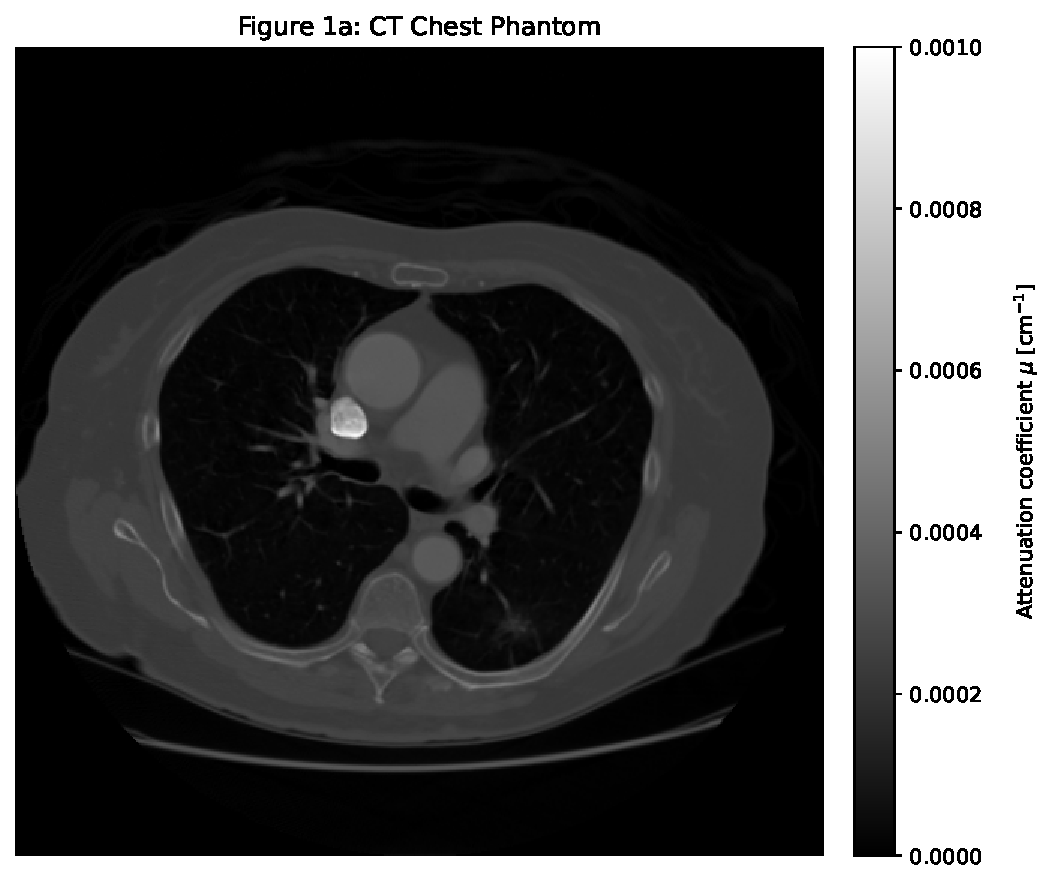
\includegraphics[width=0.7\textwidth]{figures/fig_1.1a.pdf}
    \caption{CT chest phantom with attenuation coefficients in cm$^{-1}$.}
\end{figure}

\noindent I plot the image to confirm it was loaded, and added a colourbar to show the range of attenuation coefficients. 

\subsubsection*{(b) Simulating noise and sinograms}

Gaussian ($\mu=0$, $\sigma=0.05$) and Poisson noise were simulated at three dose levels ($I_0 \in \{10^5, 10^3, 10^2\}$) for 360, 90 and 20 projections. 
The sinogram was obtained using the Radon transform and converted to Beer-Lambert transmission form, with Poisson then Gaussian noise added, and it was then converted back to an absorption sinogram.

\begin{figure}[H]
    \centering
    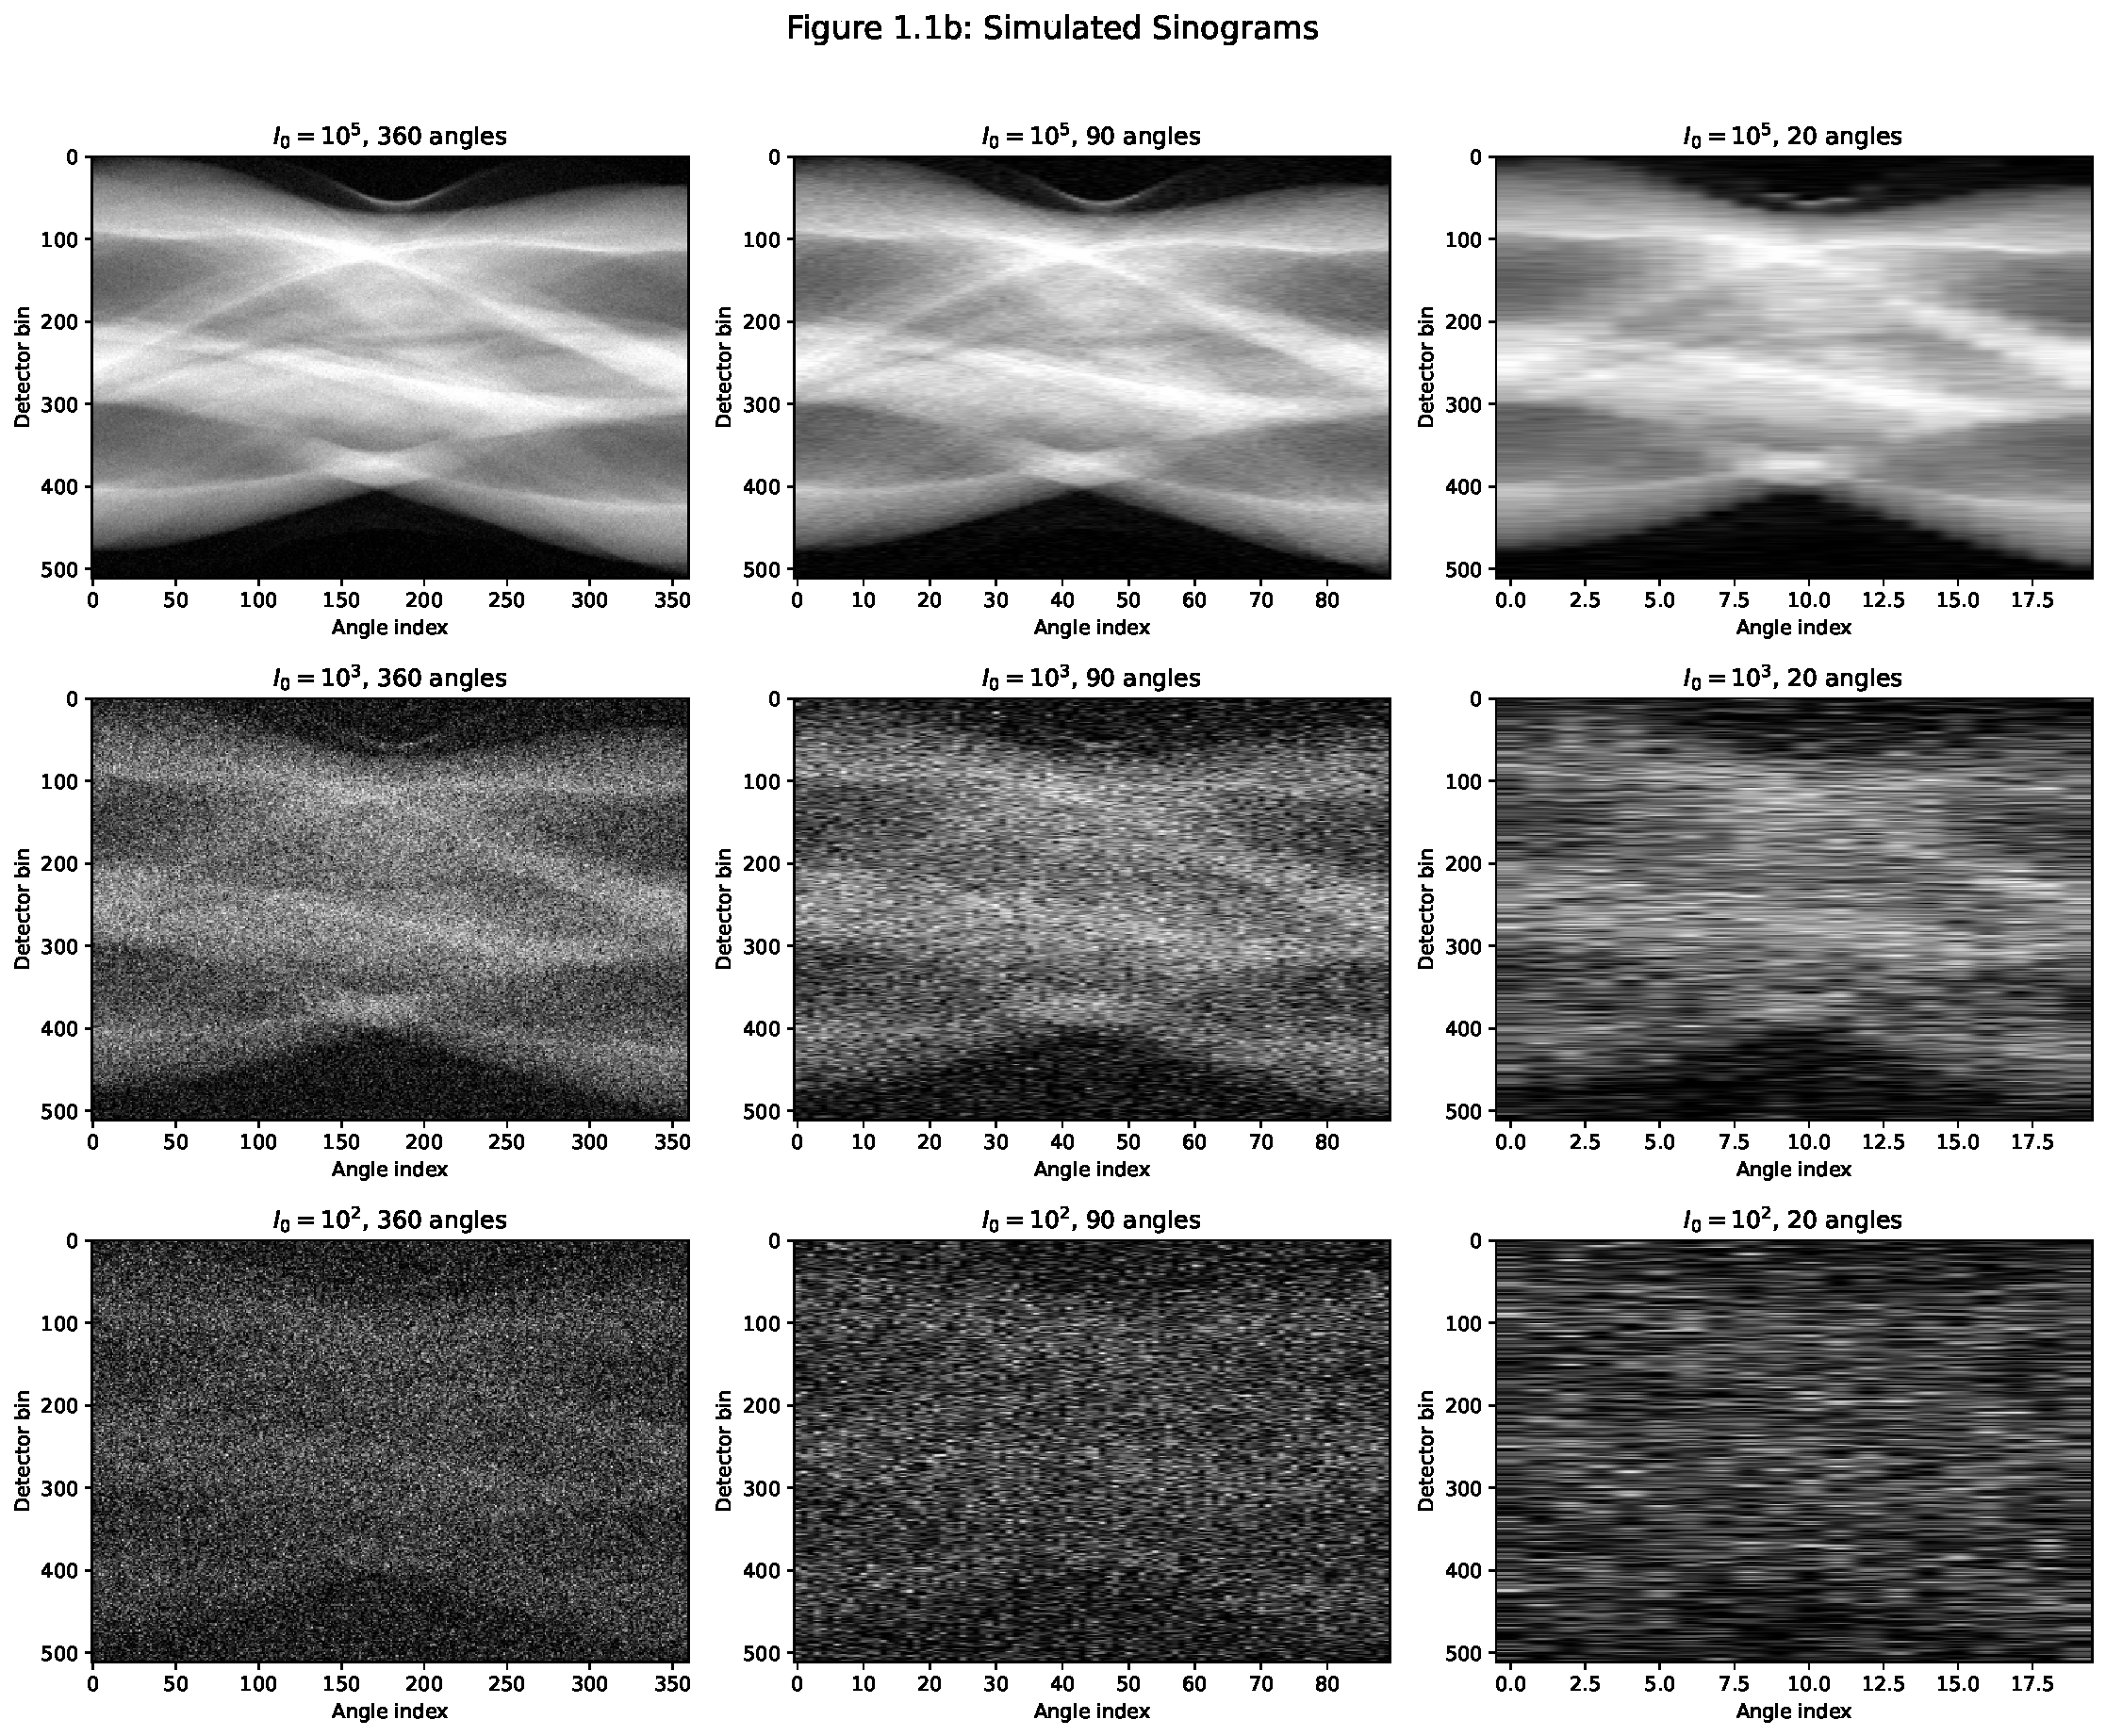
\includegraphics[width=0.95\textwidth]{figures/fig_1.1b.pdf}
    \caption{Simulated noisy sinograms across dose levels and projection counts.}
\end{figure}

\subsubsection*{(c) Reconstruction and analysis}

All sinograms were reconstructed using Filtered Back-Projection (FBP) and Gradient Descent (GD). 

\begin{figure}[H]
    \centering
    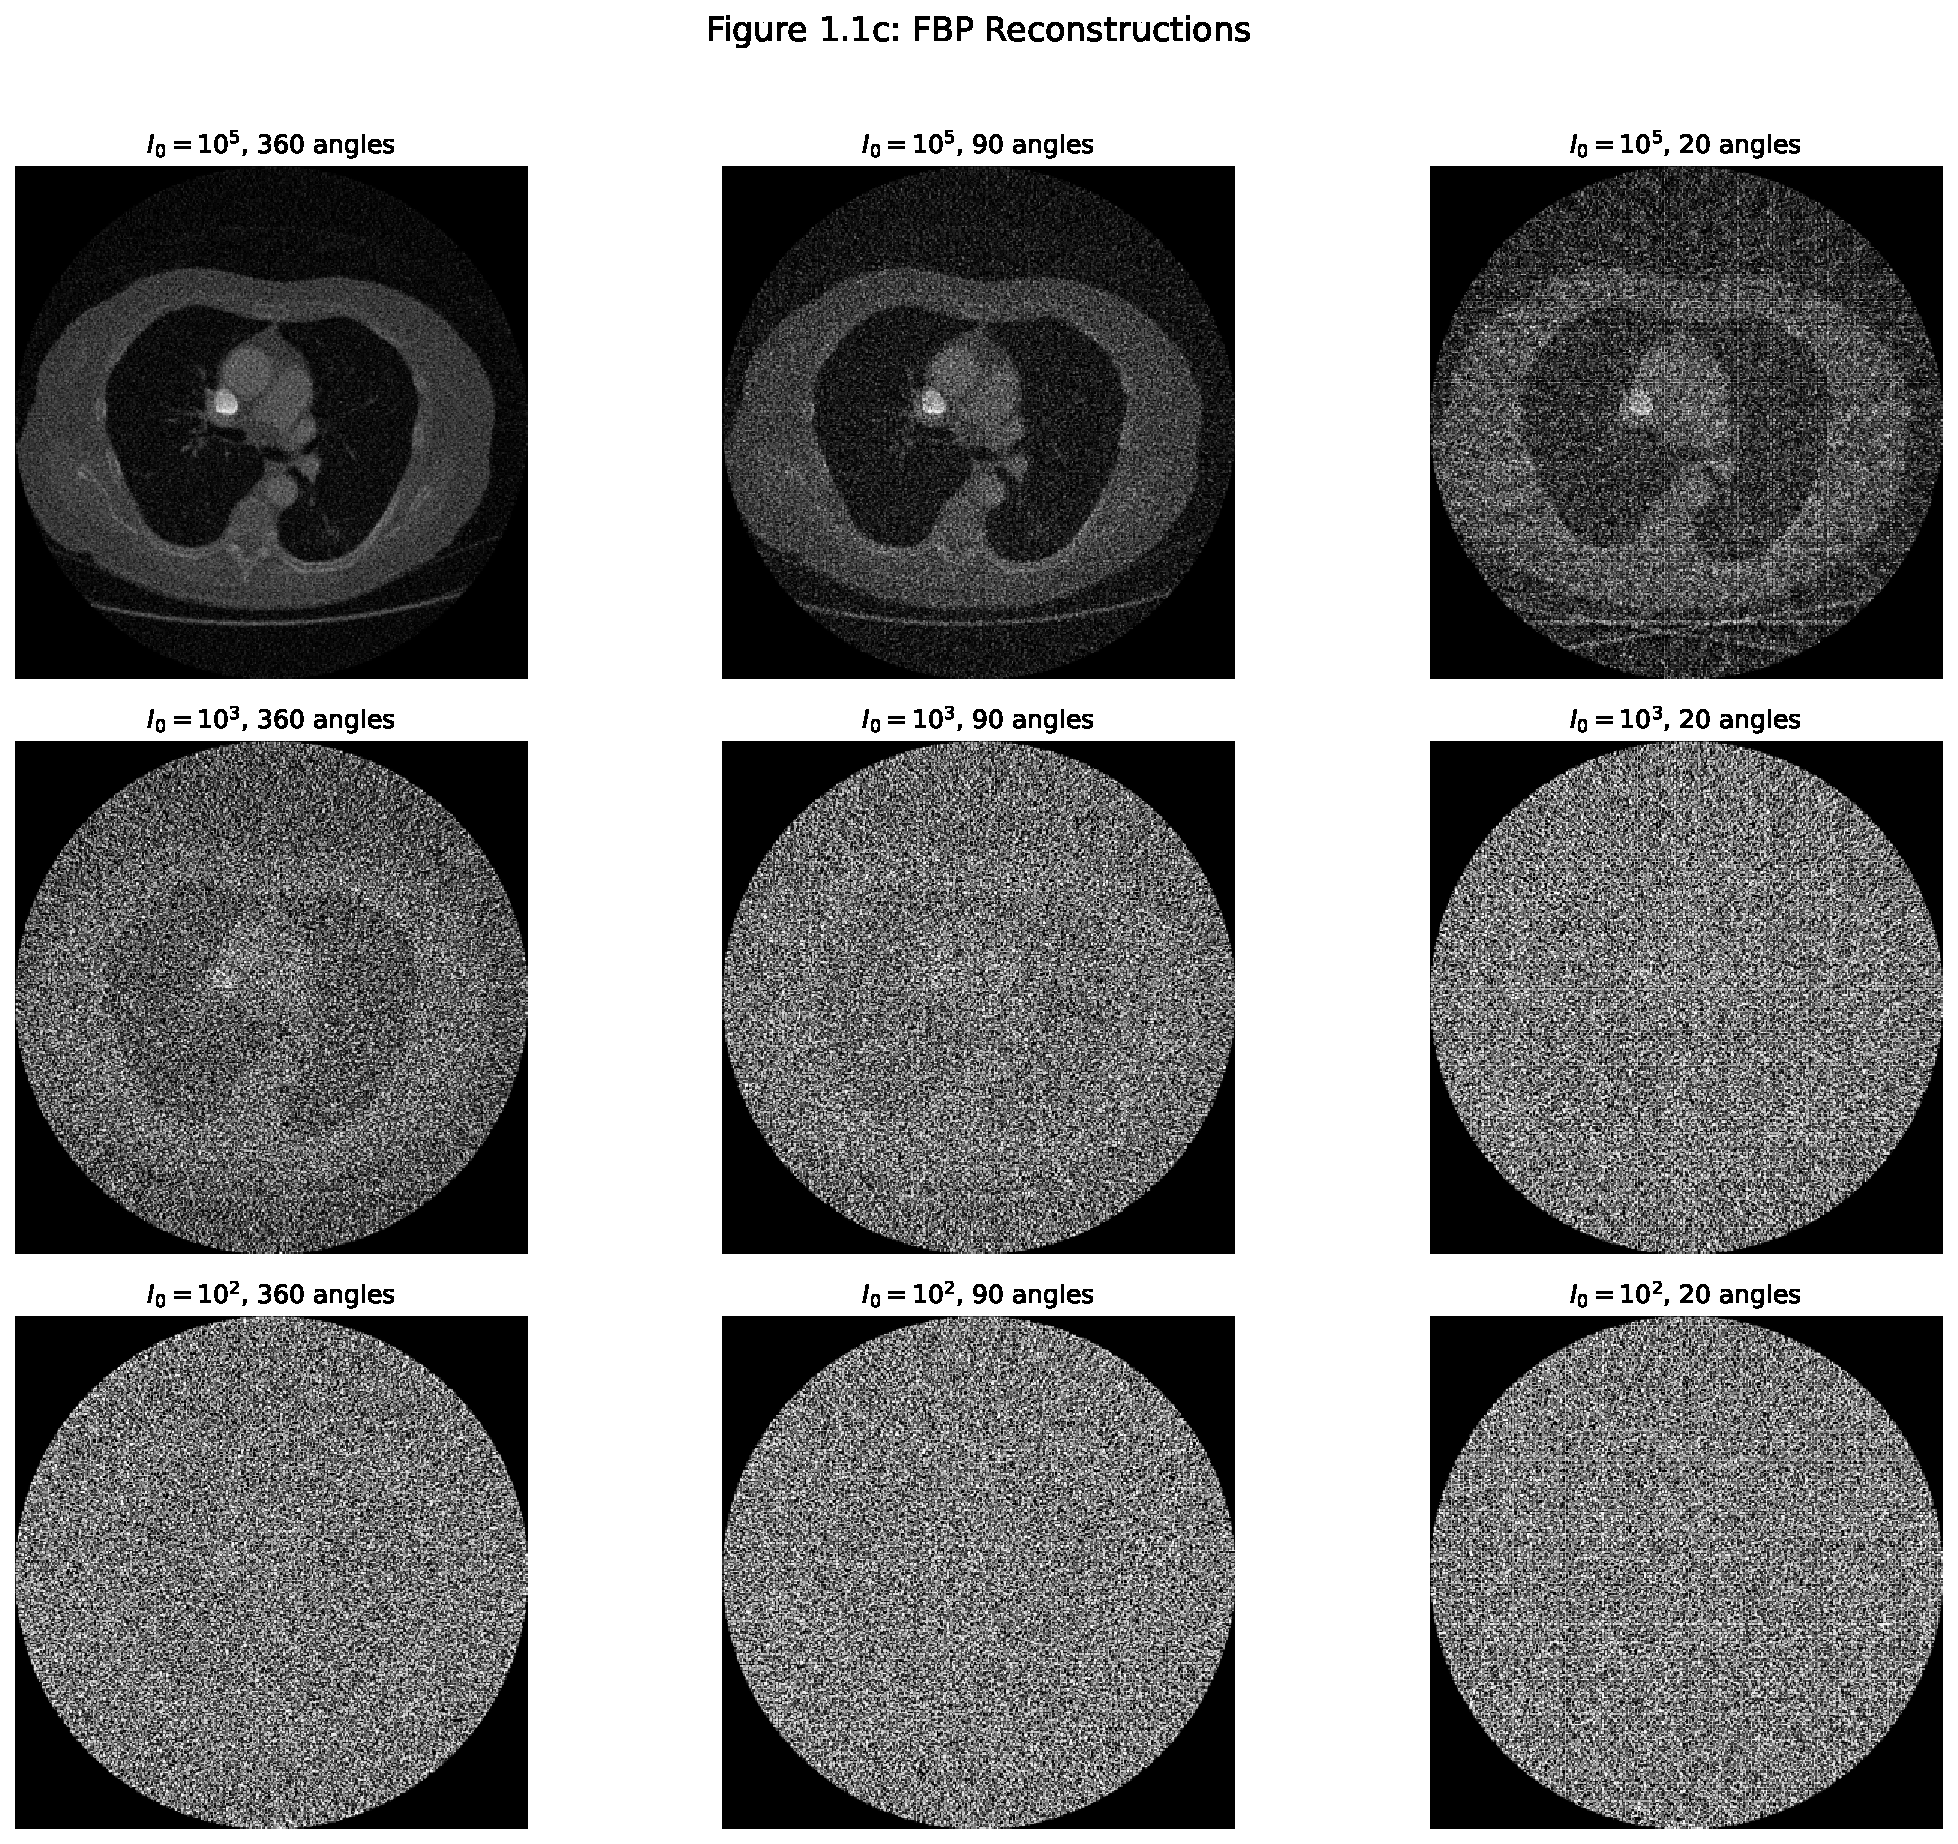
\includegraphics[width=0.7\textwidth]{figures/fig_1.1c_fbp.pdf}
    \caption{FBP reconstructions across dose levels and projection counts.}
\end{figure}

\begin{figure}[H]
    \centering
    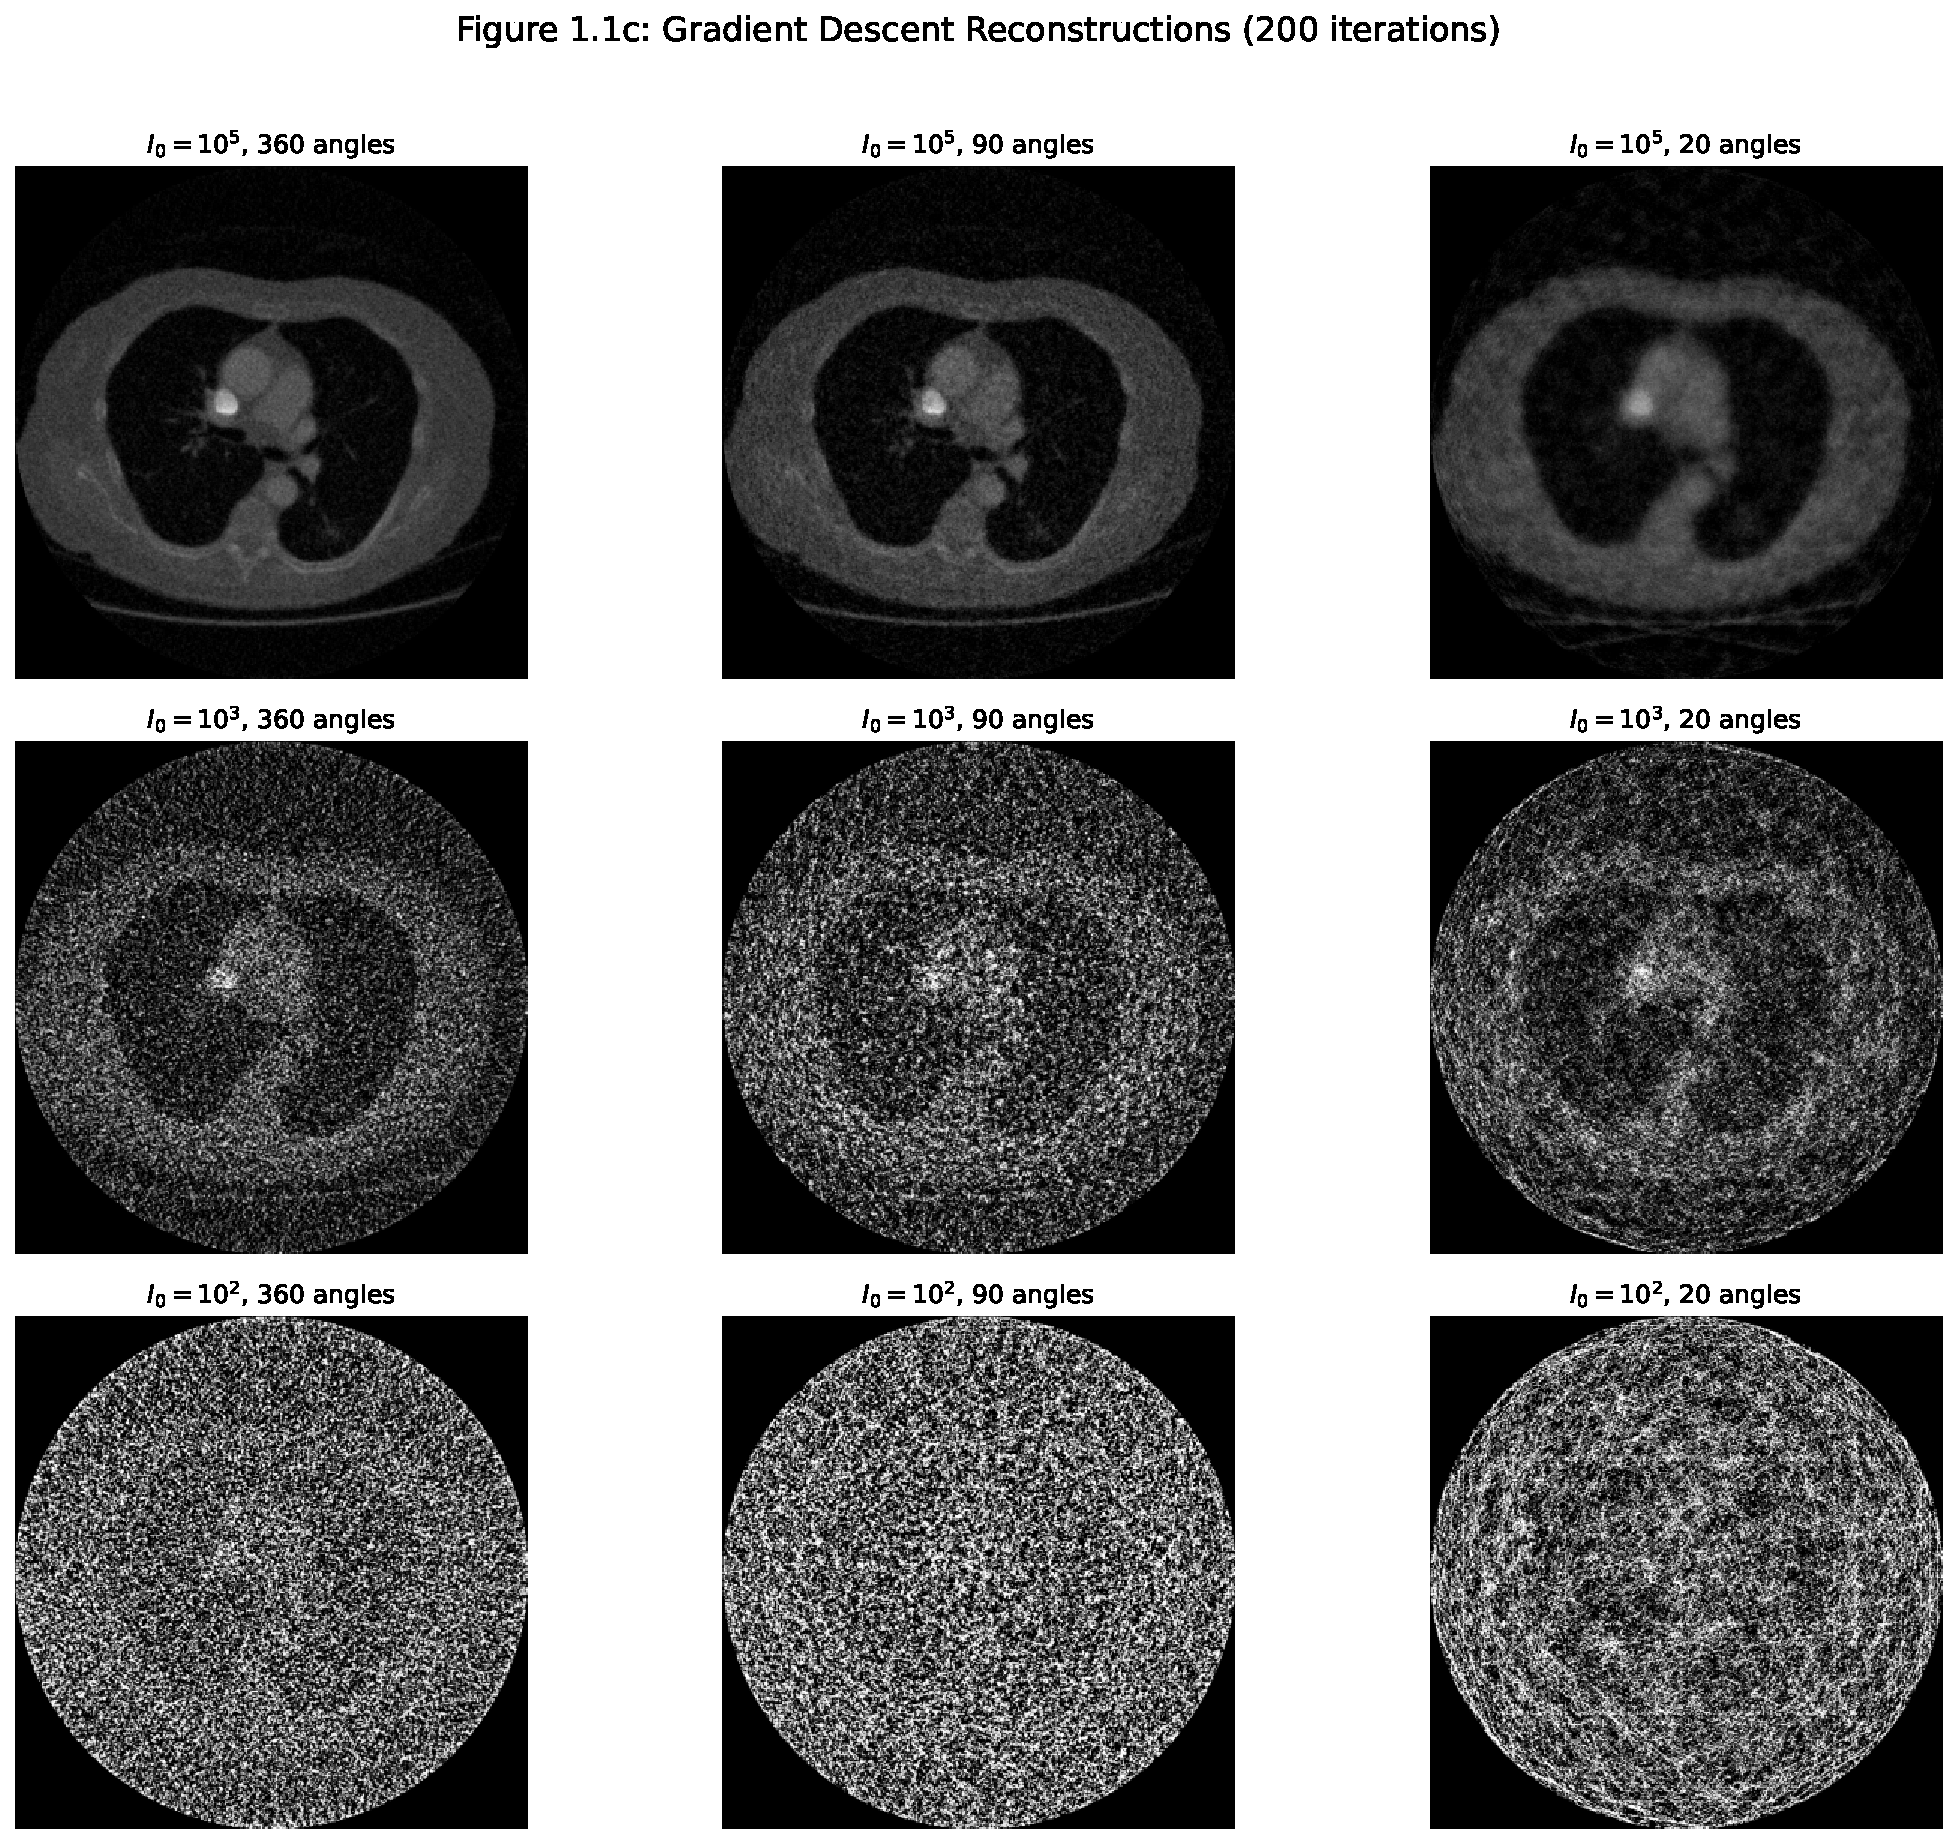
\includegraphics[width=0.7\textwidth]{figures/fig_1.1c_gd_200iter.pdf}
    \caption{Gradient Descent (200 iterations) reconstructions.}
\end{figure}

\noindent Figures 3 and 4 show the FBP and GD reconstructions. 
Comparing the two reconstruction methods, we can see that FBP works well at high dose ($I_0=10^5$), producing clear reconstructions at both 360 and 90 angles that show the anatomy and artefact correctly. 
At 20 angles, streaking begins to appear across the image due to undersampling, but the anatomy is still recognisable. 
For medium doses ($I_0=10^3$), all three reconstructions are heavily noise dominated, and the anatomy is almost entirely unrecognisable, and the case is similar for low dose ($I_0=10^2$), where all reconstructions are completely unrecognisable. \\

\noindent I decided to perform three reconstructions for Gradient Descent, of 5, 50 and 200 iterations, however in terms of performace analytics I will only focus on the 200 iteration case. 
At high dose ($I_0=10^5$), GD produced good anatomy at both 360 and 90 degrees, but with reconstructions appearing slightly softer than FBP. 
The clear difference between the two can be seen at medium dose ($I_0=10^3$), where the chest outline, its internal structures, and even the artefact are all still visible, whereas this was not the case for FBP. 
GD still struggled at low dose ($I_0=10^2$), but some structural information can still be recovered from the 360 angle plot, but overall the noise did dominate the reconstruction at this level. \\

\noindent FBP performs better when the dose is high and there is sufficient angular converage. 
It is also a single pass analytic recosntruction, meaning it is much faster and produces an image almost instantaneously. 
The default filter used in FBP is Ram-Lak, which preserves high frequency detail, resulting in images with sharp edges, critical for clinical cases. \\

\noindent However, this algorithm degrades rapidly at lower doses due to the equal amplification of high frequencies, regardless of whether they represent noise or signal. 
At lower doses, noise quickly dominates the reconstruction as the filter amplifies it just as aggresively as the true signal.\\

\noindent GD performs better when dose is reduced. It does not amplify noise in the same way as FBP, but fits sinogram data progressively resulting in better oerformance at that level. 
It also does better when angular coverage is sparse, handling undersampled data much better than FBP which produces streaks from incomplete coverage. \\

\noindent The reconstructions from GD are softer than FBP as the images are built up from zero initialisations with no sharpening filter. 
Edge sharpness is extremely important in clinical CT, so FBP outperforms here. \\

\noindent A key point to note is the trade off between the two algorithms concerning computational cost. 
FBP produces images instantly, whereas GD takes time to perform iterations, increasing the more we do. 
This poses a significant difference in clinical settings, but also creates an important dilemma for GD, as shown in the plots, because choosing a small number of iterations for a short compute time produces bad quality reconstructions, and the opposite applies for larger numbers of iterations. \\

\begin{figure}[H]
    \centering
    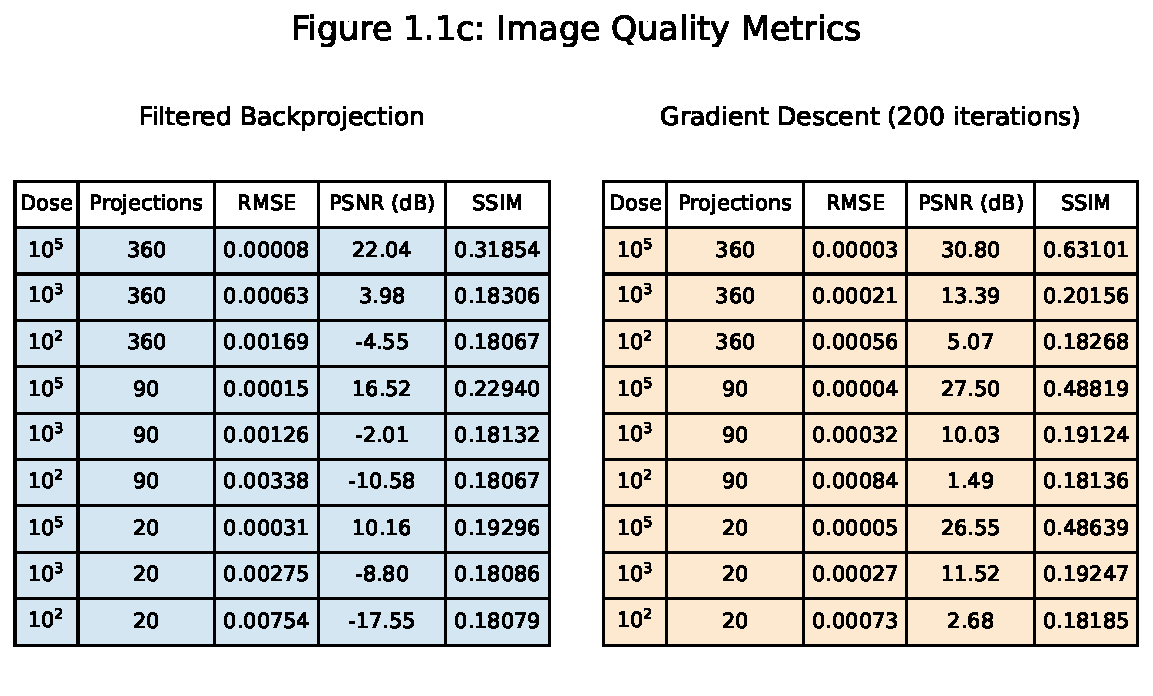
\includegraphics[width=0.9\textwidth]{figures/fig_1.1c_metrics.pdf}
    \caption{Image quality metrics (RMSE, PSNR, SSIM) for FBP and GD.}
\end{figure}

\begin{figure}[H]
    \centering
    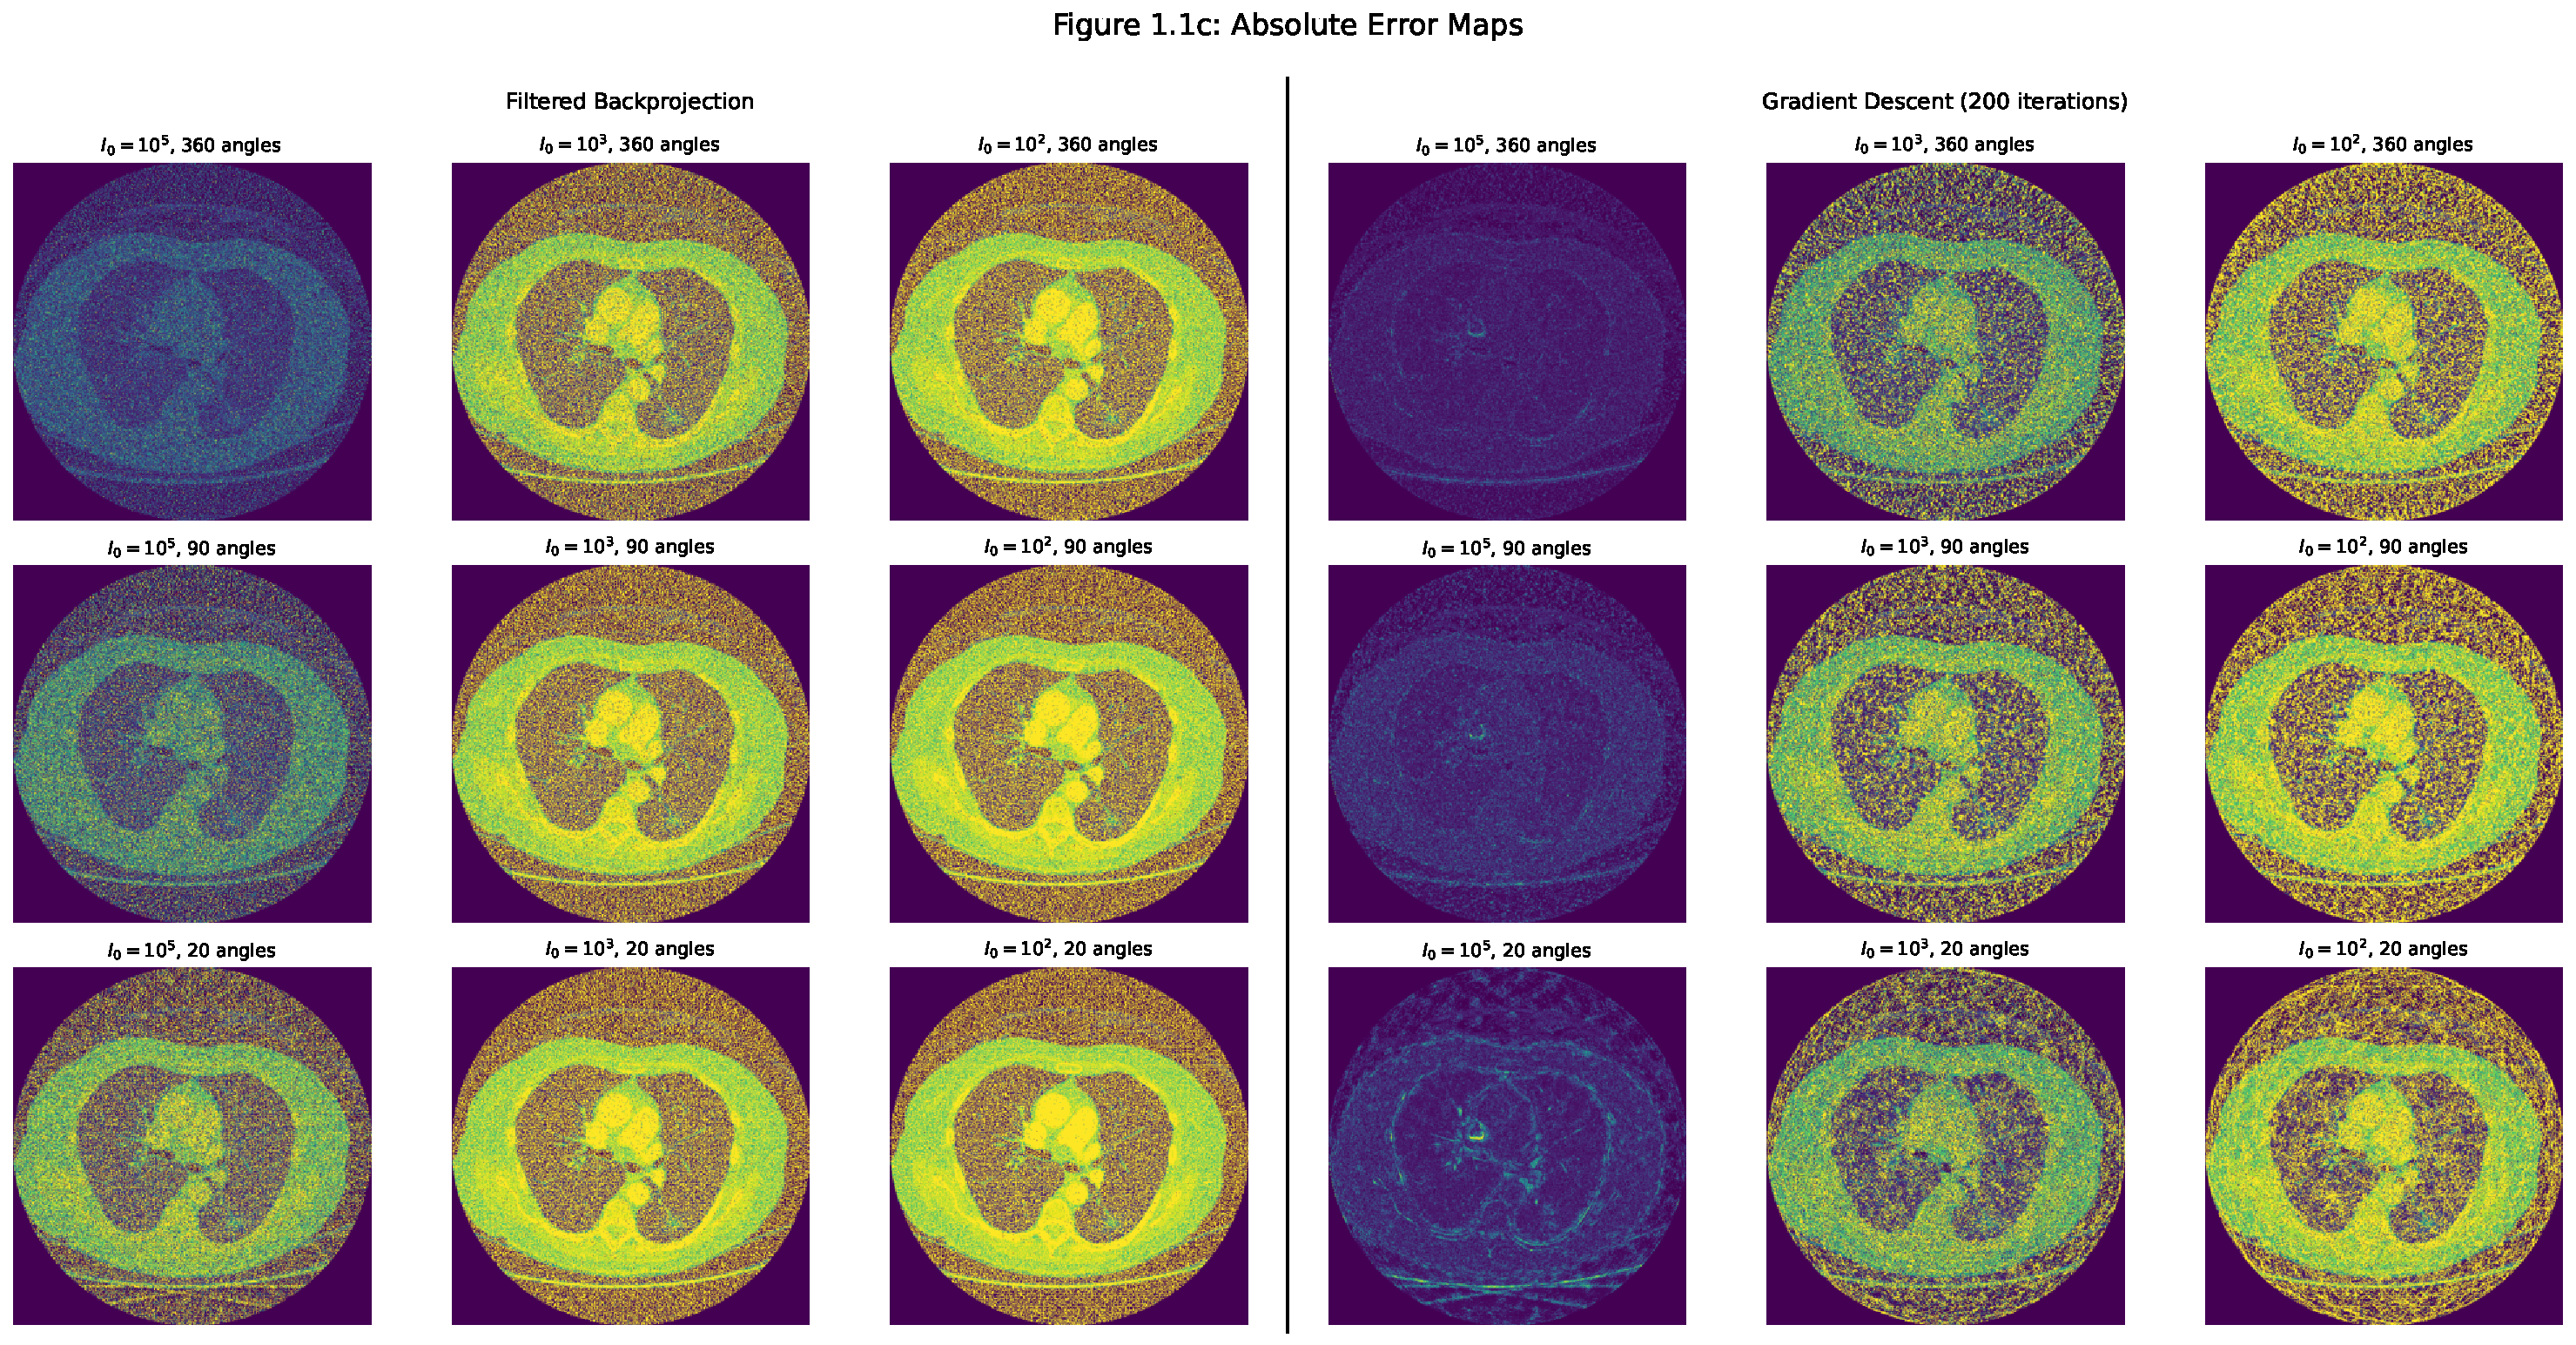
\includegraphics[width=0.9\textwidth]{figures/fig_1.1c_errors.pdf}
    \caption{Absolute error maps for FBP and GD reconstructions.}
\end{figure}

\noindent Reducing the source intensity ($I_0$) directly reduces the radiation dose delivered to the patient, which is important as X-rays are a form of ionising radiation, and can damage DNA is there is enough exposure. CT is one of the highest dose forms of medical imaging, so being able to limit the dose of radiation received has a meaningful impact on patient safety, especially for patients with chronic or long term conditions receiving many scans. The trade off here is that as the dose is lowered, it becomes very difficult to reconstruct, which can be seen from our plots where at $I_0 = 10^2$ neither algorithm can produce acceptable images. \\

\noindent Reducing the number of projections shortens the total scan time, which not only reduces patient discomfort or anxiety, but also reduces motion artefacts, as patients will not move or breathe as much during a shorter scan. This is valuable for CTs of constantly moving organs such as the heart, but also for paediatric cases, where children find it much harder to remain still or to perform actions such as holding their breath. Despite these advantages, sparse view CT introduces streak artefacts, which can clearly be seen in the plot for our 20 angle reconstructions. If these artefacts were to appear over the patient's organs, they could be misinterpreted as lesions or hide real ones.\\

\noindent FBP produces instant results, along with sharp and high quality images at standard doses with enough angles. In clinical practice this means that reconstructions are available straight away, and show all boundaries and edges clearly. This is vital in emergency situations where clinicians are unable to wait for scans and need them to be ready straight away. The disadvantage of FBP is that results are extremely sensitive to dose reduction, so are unstable for low dose CT. \\

\noindent Gradient Descent can withstand noise and sparse data better than FBP, but comes at a significant computational cost, as enough iterations need to be performed in order to acheive adequate reconstructions, but the more reconstructions we do the more time it takes, with 200 iterations taking approximately 8 minutes on my machine. In clinical practice this is addressed through the use of GPU accelerated implementations, but these still do not acheive that instant reconstructions that FBP does. Another issue with GD is the softer appearance of edges, which arises from building the image gradually through iterations, without the use of a sharpening filter. This is a disadvantage in clincial imaging, as sharp edges are crucial for detecting anatomy and its margins, as well as performing measurements. \\

\noindent The comparison of scanning procedures and reconstruction algorithms has a direct impact of their applications in CT scanning protocols for clinical practice. Reducing $I_0$ from $10^5$ to $10^3$ represents a $100\times$ reduction in radiation dose, which has an enourmous impact for patients who undergo regular scans as part of their treatment. Being subjected to a lower dose each time significantly reduces the radiation the patients are exposed to, and therefore the risk of cancer or other exposure related complications. However, as demonstrated by the FBP results, reducing dose significantly impacts image reconstruction, meaning that while low dose CT is exceptionally meaningful, it is only a viable option when paired with iterative or deep learning reconstructions. \\

\noindent Reducing angle projections from 360 to 20 cuts the scan time by approximately $18\times$. This kind of reduction is very important for instances like cardiac or paediatric CT scans, where scans must be completed as quickly as possible before they are destroyed by motion. This is also meaningful for emergency imaging, where faster imaging results in faster diagnosis and treatment. This is however balanced with an increase in streak artefacts and the loss of fine details, which may be acceptable in certain scanerios, but not in cases where the radiologist is relying on these details to make a diagnostic decision. \\

\noindent The choice of algorithm also has a clear impact on the outcome. FBP's near instant results are critical in time sensitive settings like emergency medicine, but suffer when dose is reduced, whereas GD produces better quality images at reduced doses, but requires significantly more computation and time, which is ideal when low dose is necessary, but the results aren't needed urgently.\\

\subsubsection*{(d) Methods for improvement}

\noindent Adding a regulariser to the Gradient Descent minimisation problem helps encode prior knowledge about what the final image should look like. One example is Total Variation, which turns the problem into the following:

$$\hat{\mu} = \arg\min_\mu \|A\mu - p\|^2 + \alpha R(\mu)$$

\noindent where the regularisation term is:

$$TV(\mu) = \|\nabla\mu\|_1 = \sum_{i,j} \sqrt{|\mu_{i,j+1} - \mu_{i,j}| + |\mu_{i+1,j} - \mu_{i,j}|}$$

\noindent TV penalises the sum of image gradients, which promotes piecewise constant solutions with sharp edges, directly addressing the noise seen in our reconstructions, but still maintaining anatomical boundaries. Aside from TV, we can also use L1 or L2 norms as regularisers in reconstruction problems. \\

\noindent We can also implement Deep Learning denoising, which involves training a model such as a UNet, GAN, Diffusiion model etc. to learn an improved image from a worse one. This allows reconstructions to still use FBP and acheive instant results when needed, but then be passed through a model to reduce noise and improve quality. While this is very computationally efficient and versatile, the method relies heavily on its trainig data, and can be subject to hallucinations, where the model may remove or add artefacts from the image and affect the patient's diagnosis. \\

\noindent Non-Local means is another denoising method, which can be applied as a regulariser but also in post-processing. NLM will search the entire image to find patches with a similar structure and average them together, before replacing this average into the original patches. It is very useful for reducing noise while preserving texture and and structural details, so is better than local filtering methods. The trade off is the computational cost, as it is significantly more demanding than simpler methods.\\

% ──────────────────────────────────────────────
\subsection*{Exercise 1.2: Limited Angle Tomography}

\subsubsection*{(a) Simulating limited angle sinograms}

Noisy sinograms were simulated at three angular ranges (180\textdegree, 120\textdegree, 40\textdegree) with fixed high dose $I_0=10^5$ to isolate the effect of limited angular coverage.

\begin{figure}[H]
    \centering
    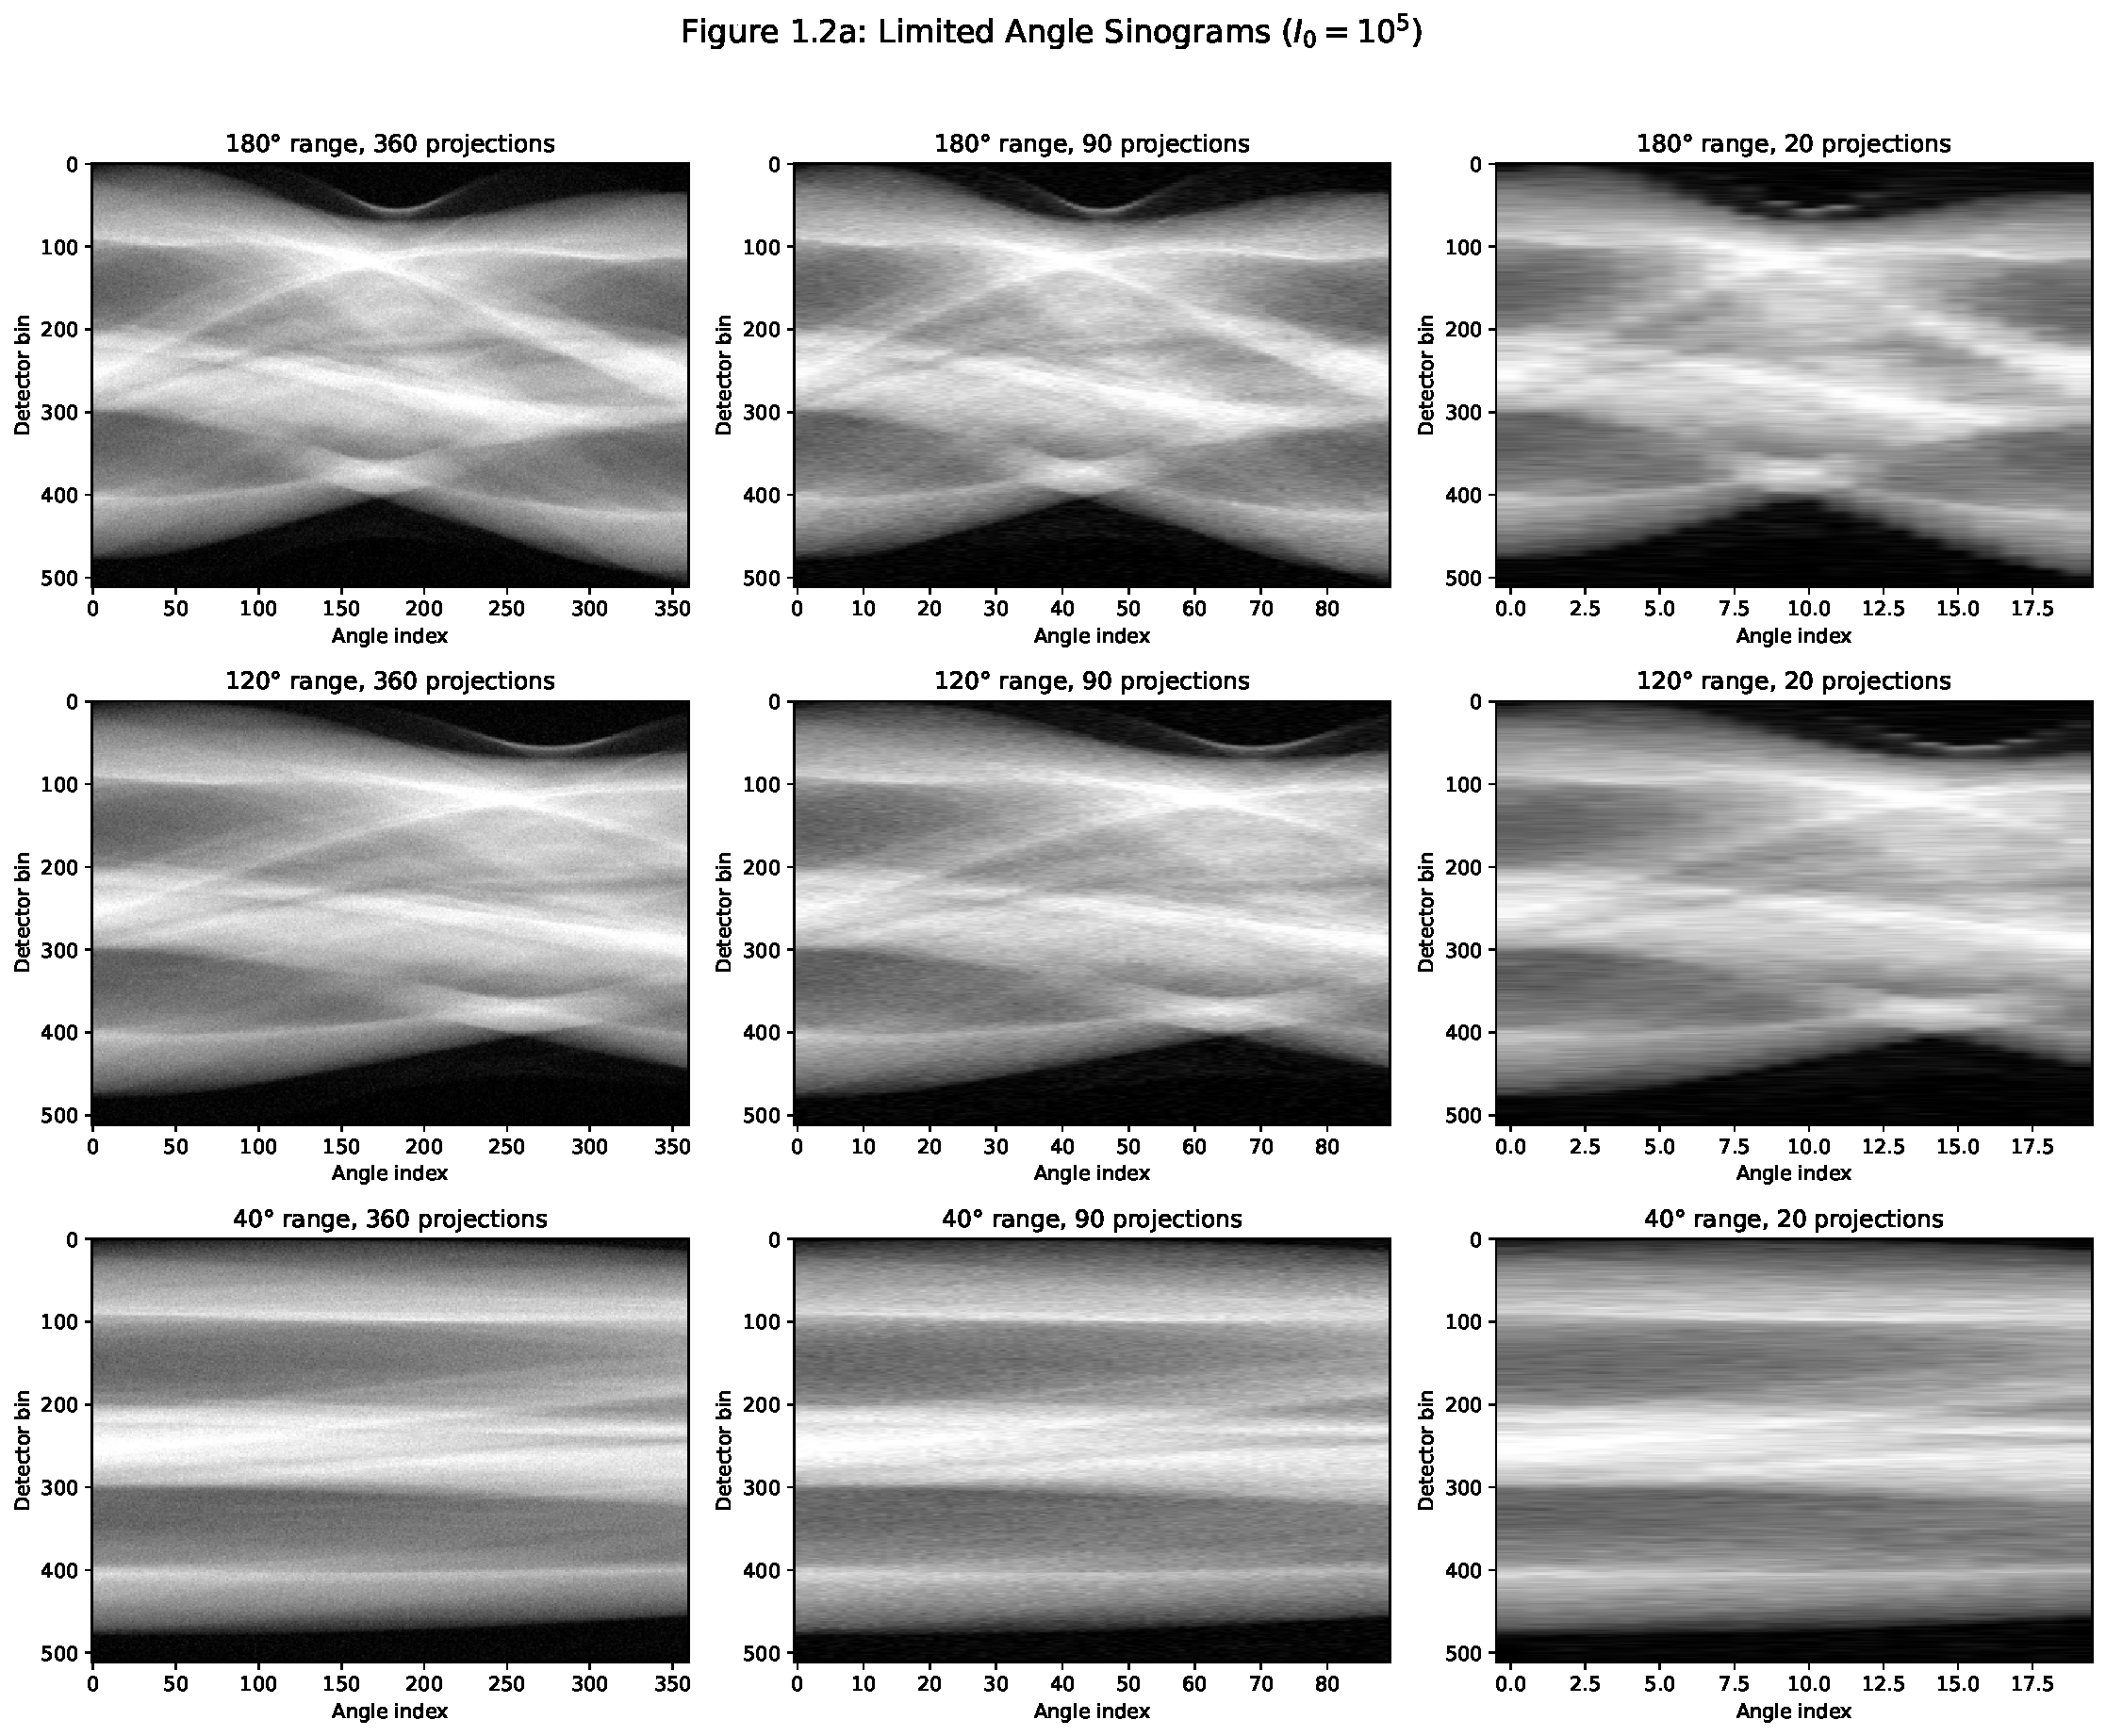
\includegraphics[width=0.7\textwidth]{figures/fig_1.2a.pdf}
    \caption{Limited angle sinograms at $I_0=10^5$.}
\end{figure}

\subsubsection*{(b) Limited angle reconstructions}

\begin{figure}[H]
    \centering
    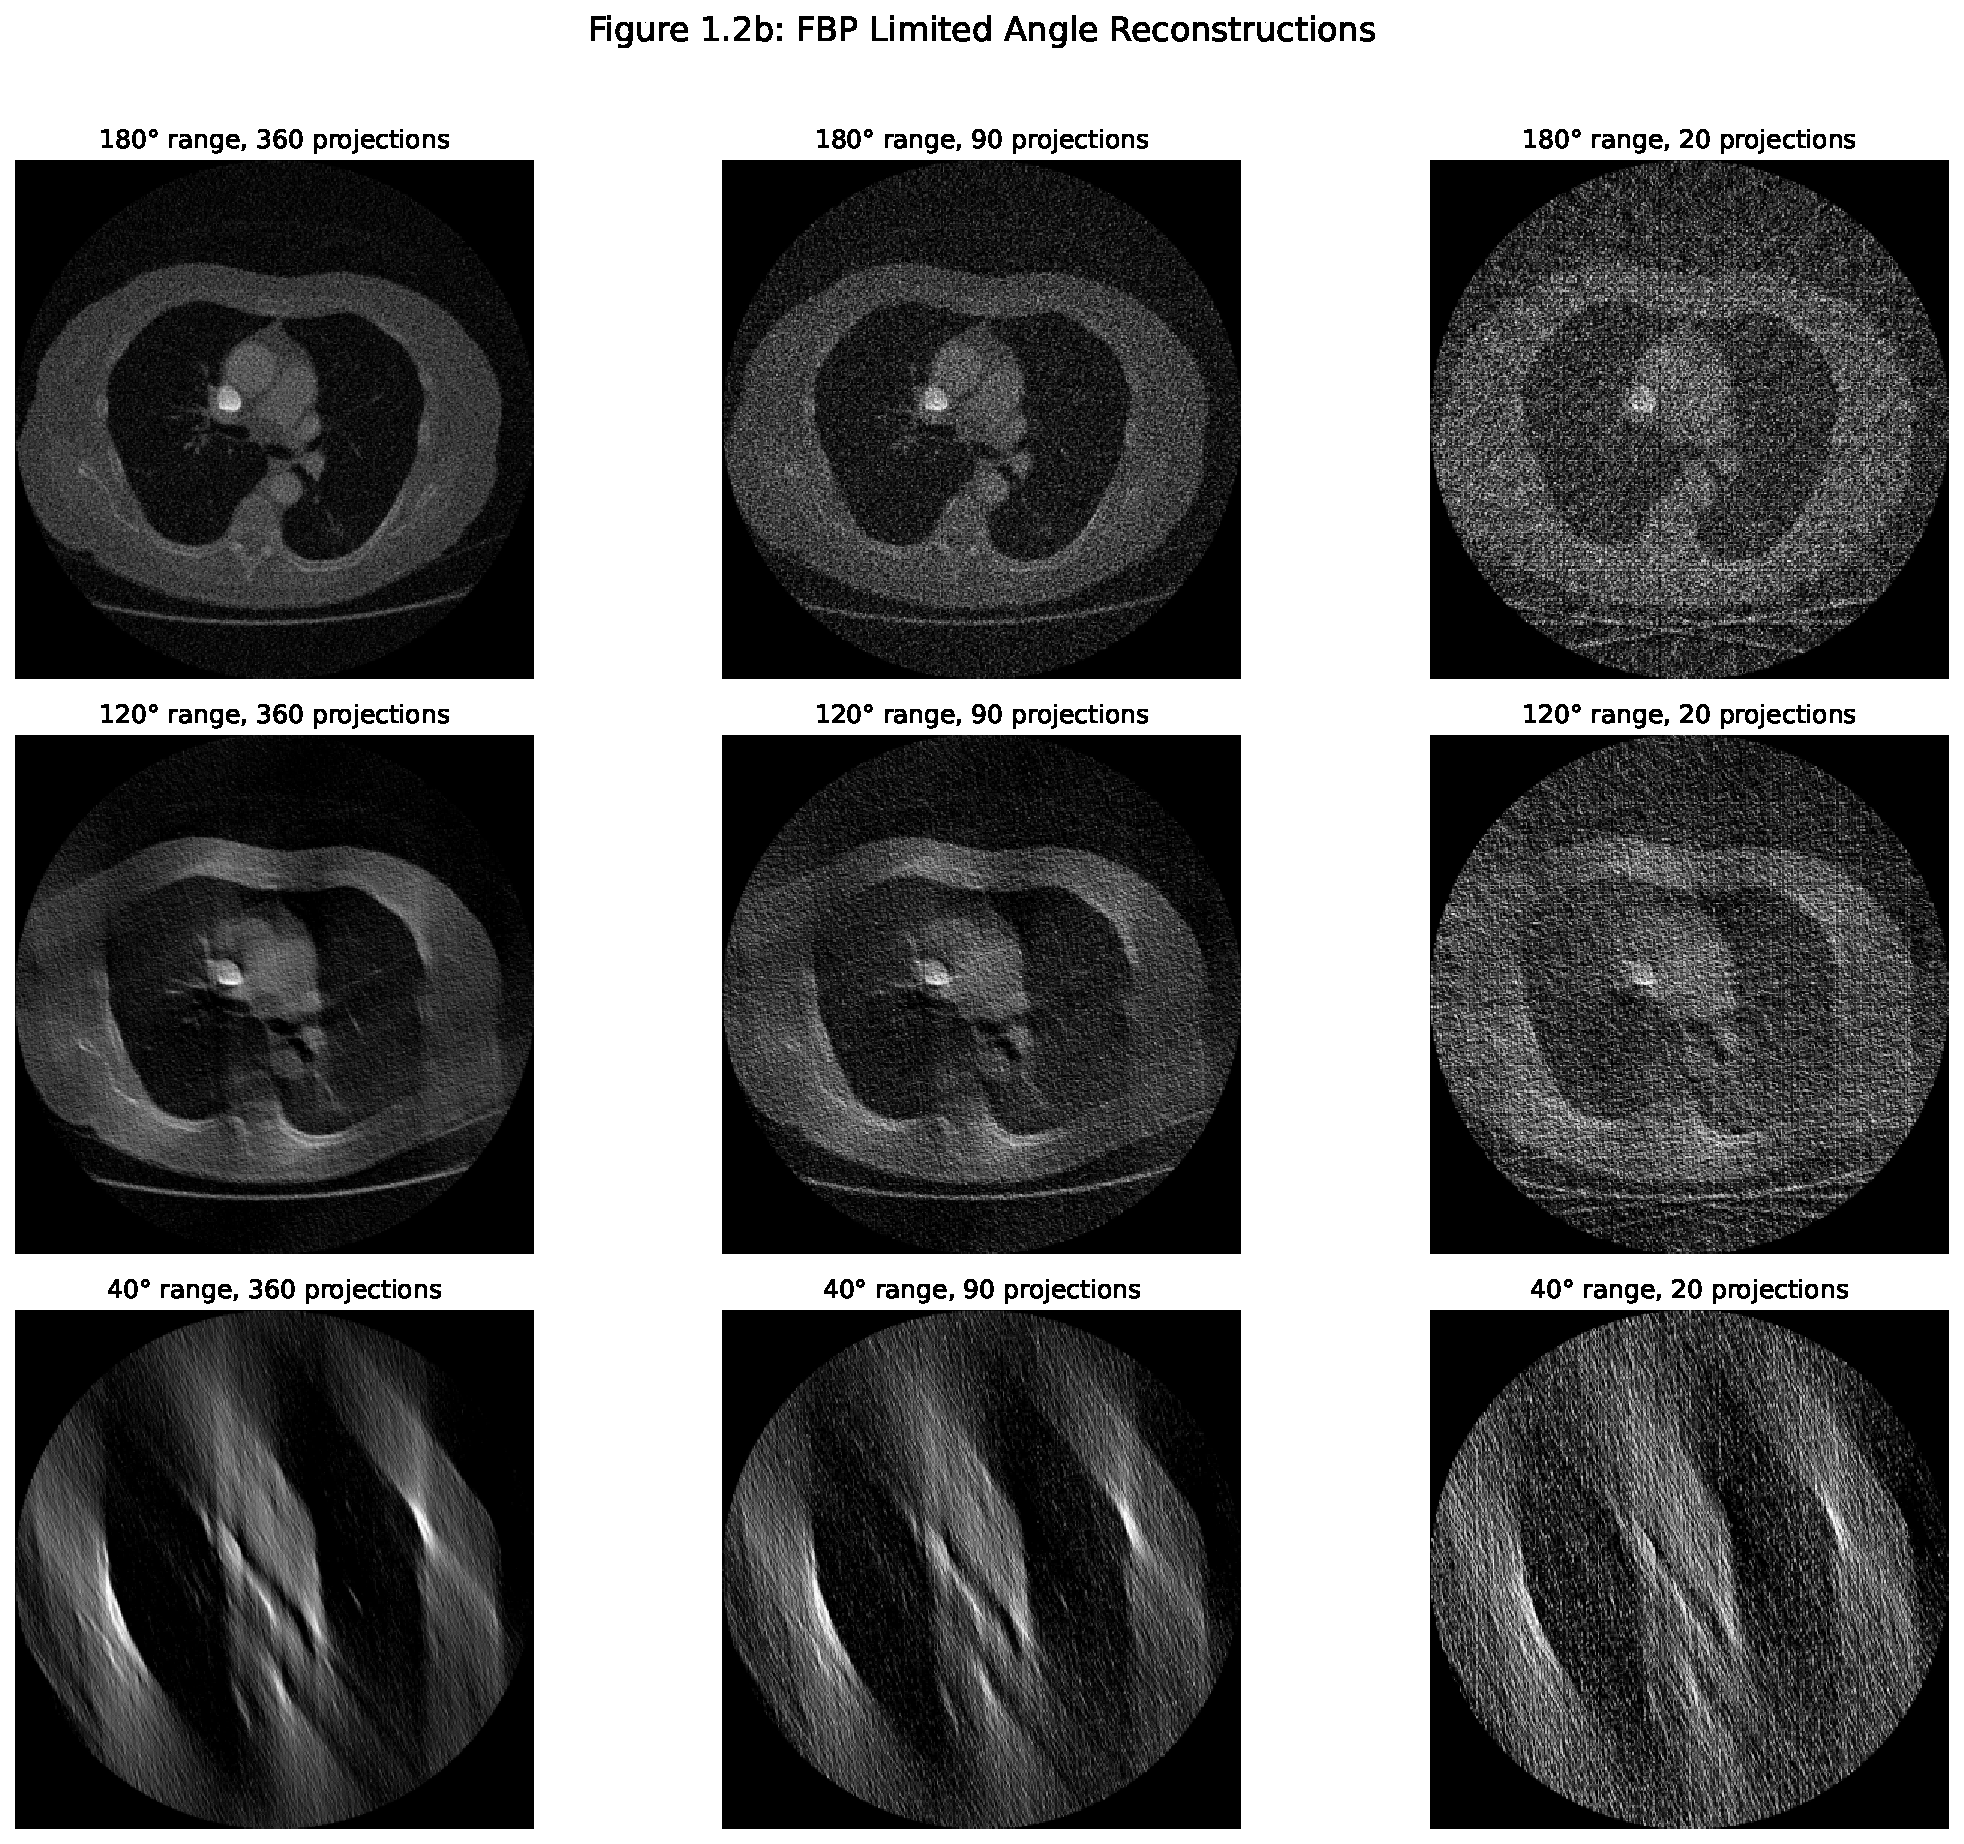
\includegraphics[width=0.7\textwidth]{figures/fig_1.2b_fbp.pdf}
    \caption{FBP reconstructions for limited angle sinograms.}
\end{figure}

\begin{figure}[H]
    \centering
    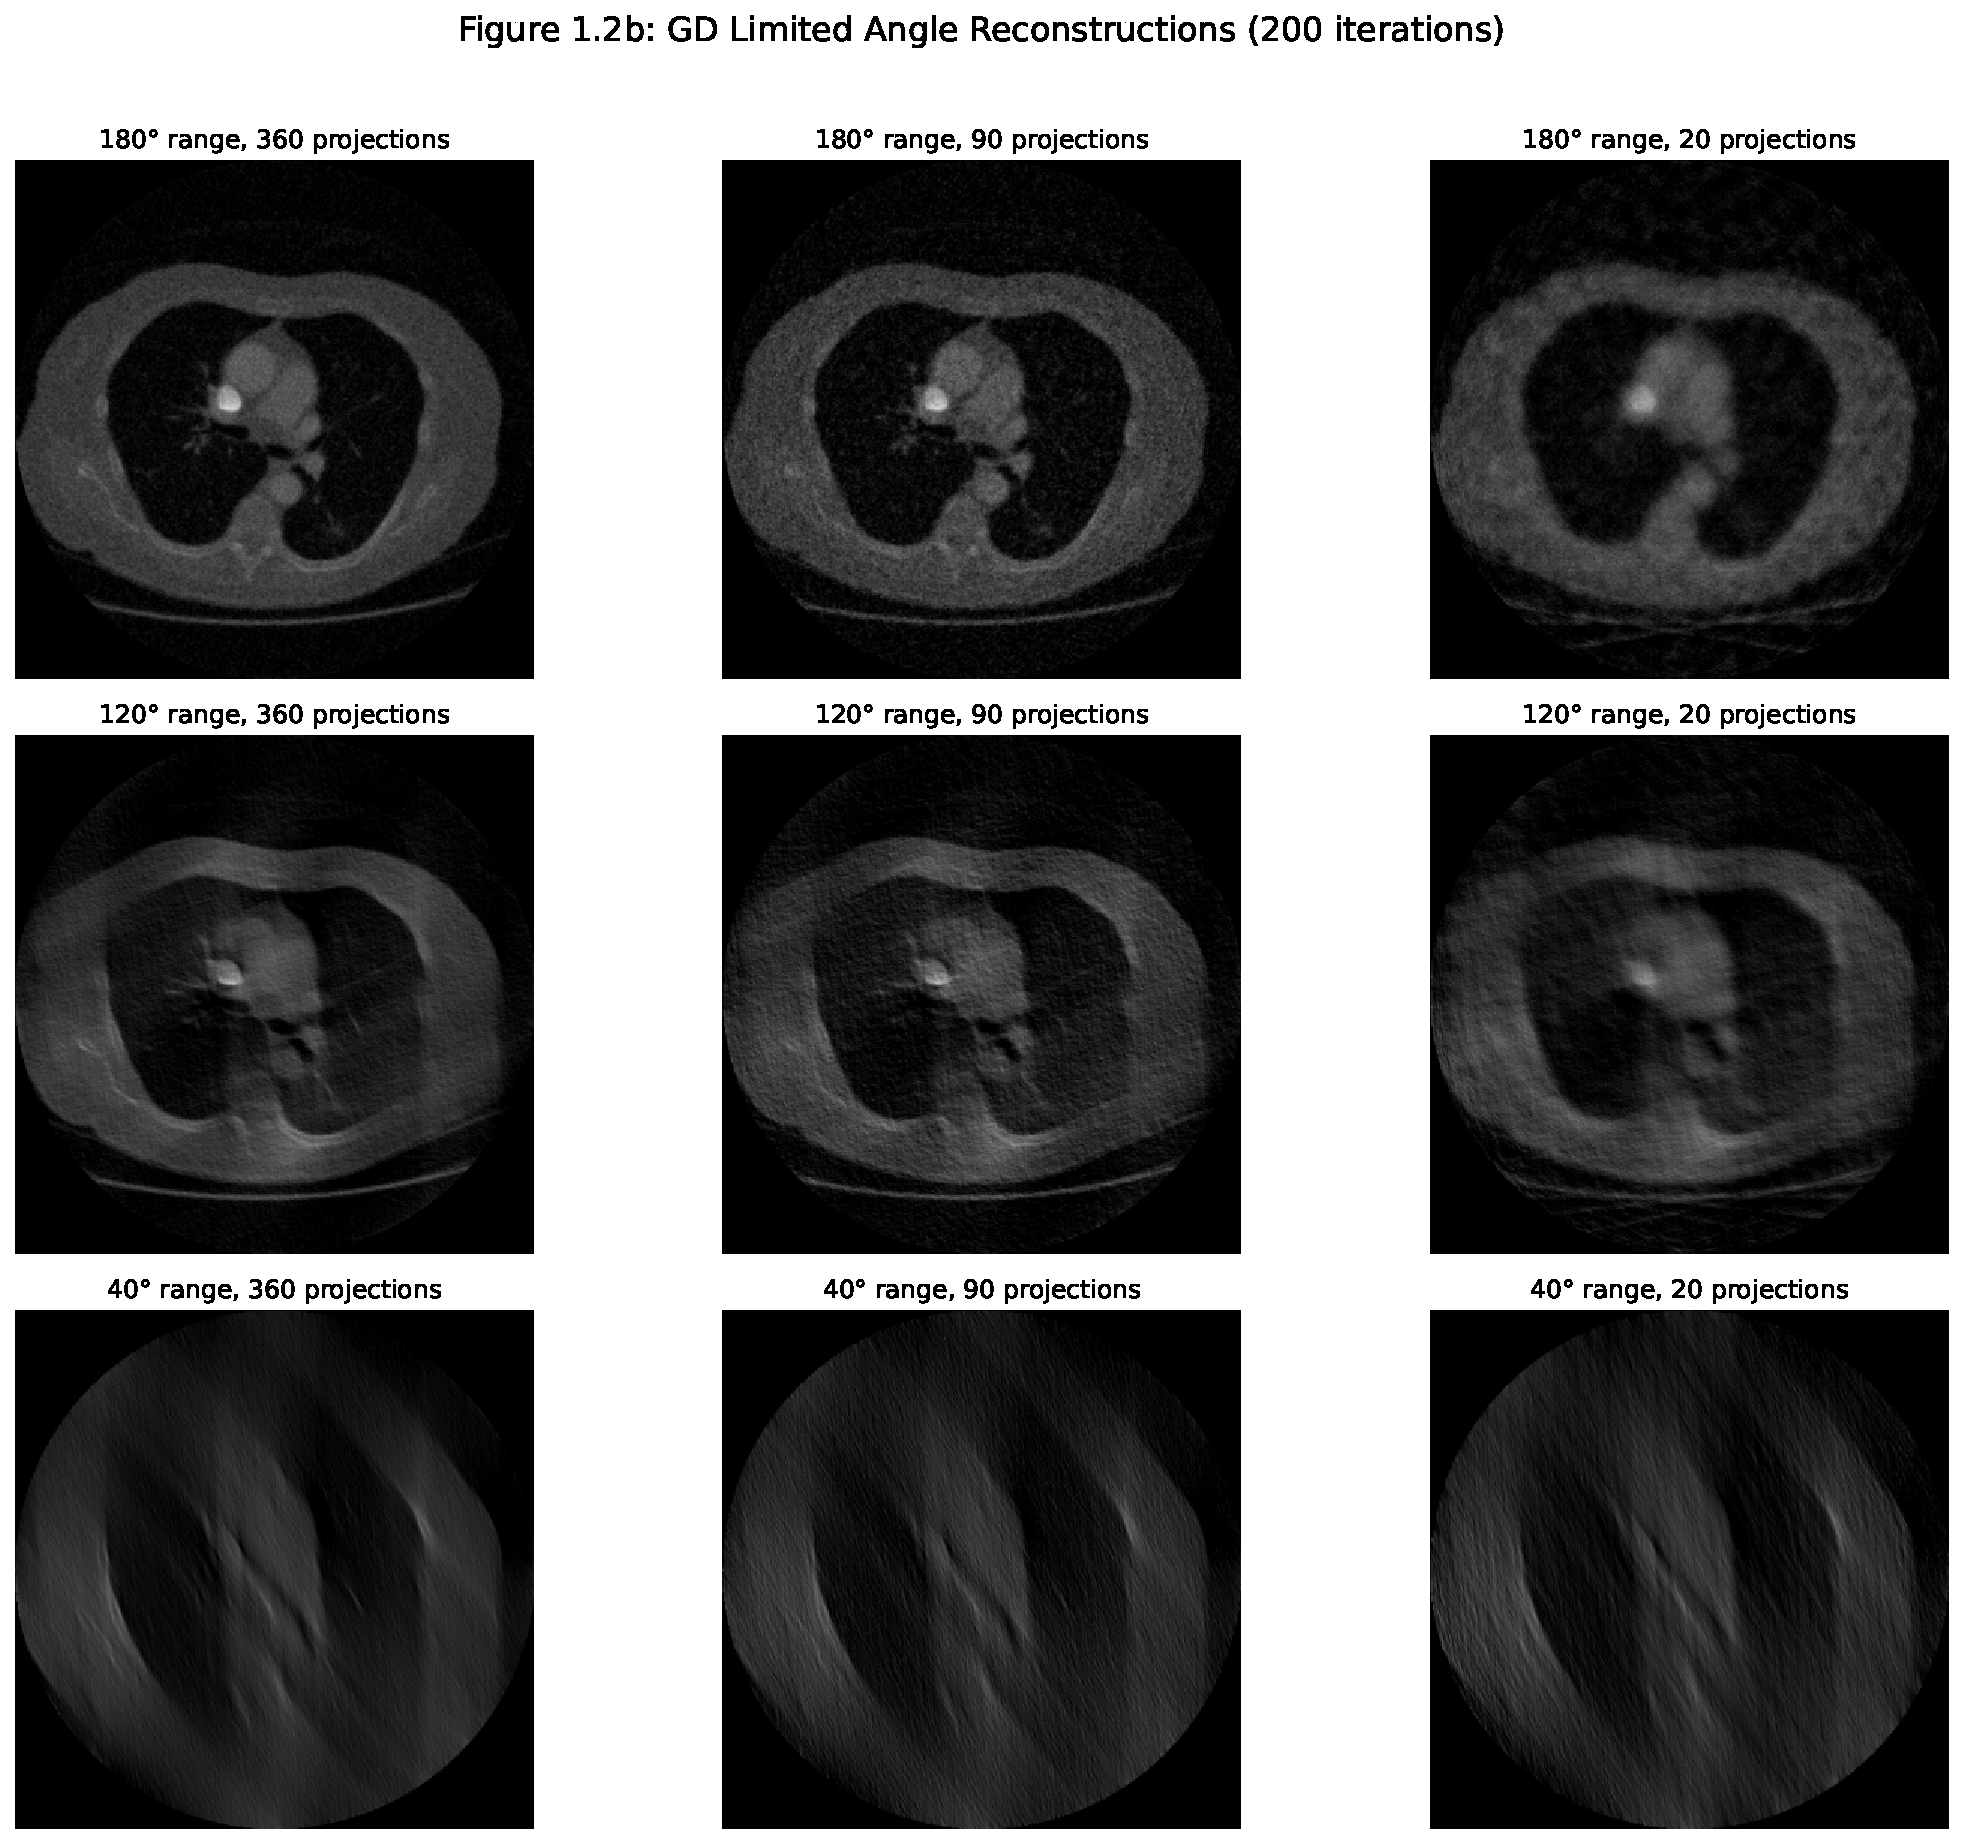
\includegraphics[width=0.7\textwidth]{figures/fig_1.2b_gd.pdf}
    \caption{GD reconstructions for limited angle sinograms.}
\end{figure}

\begin{figure}[H]
    \centering
    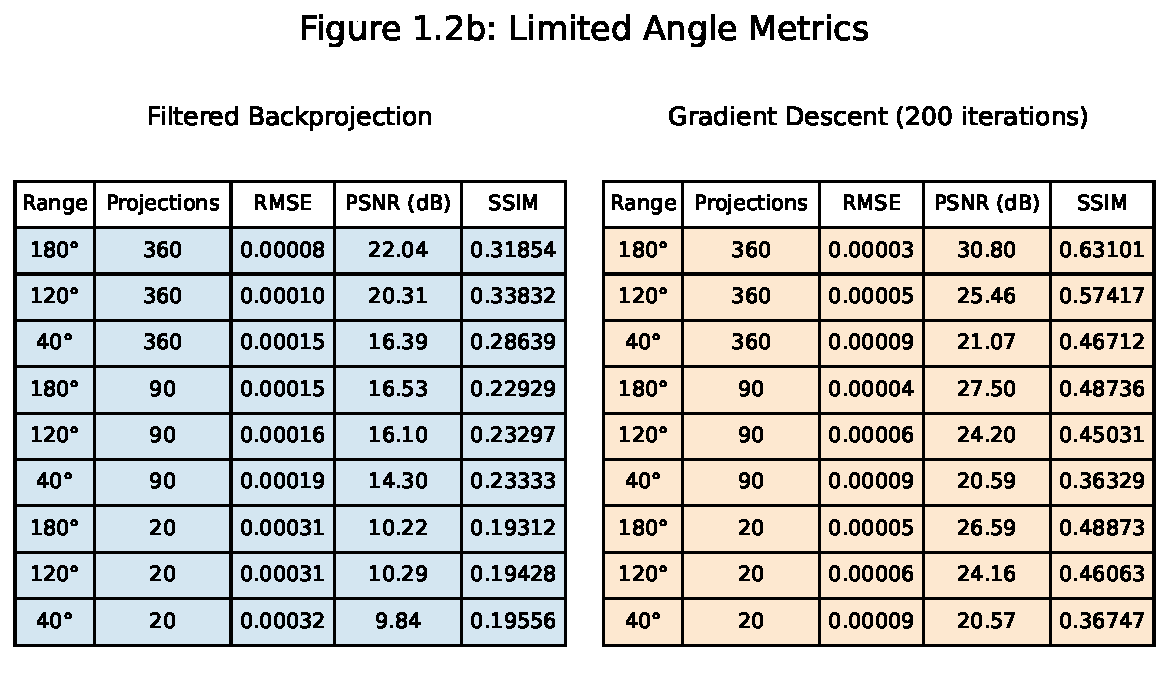
\includegraphics[width=0.9\textwidth]{figures/fig_1.2b_metrics.pdf}
    \caption{Limited angle image quality metrics.}
\end{figure}

\begin{figure}[H]
    \centering
    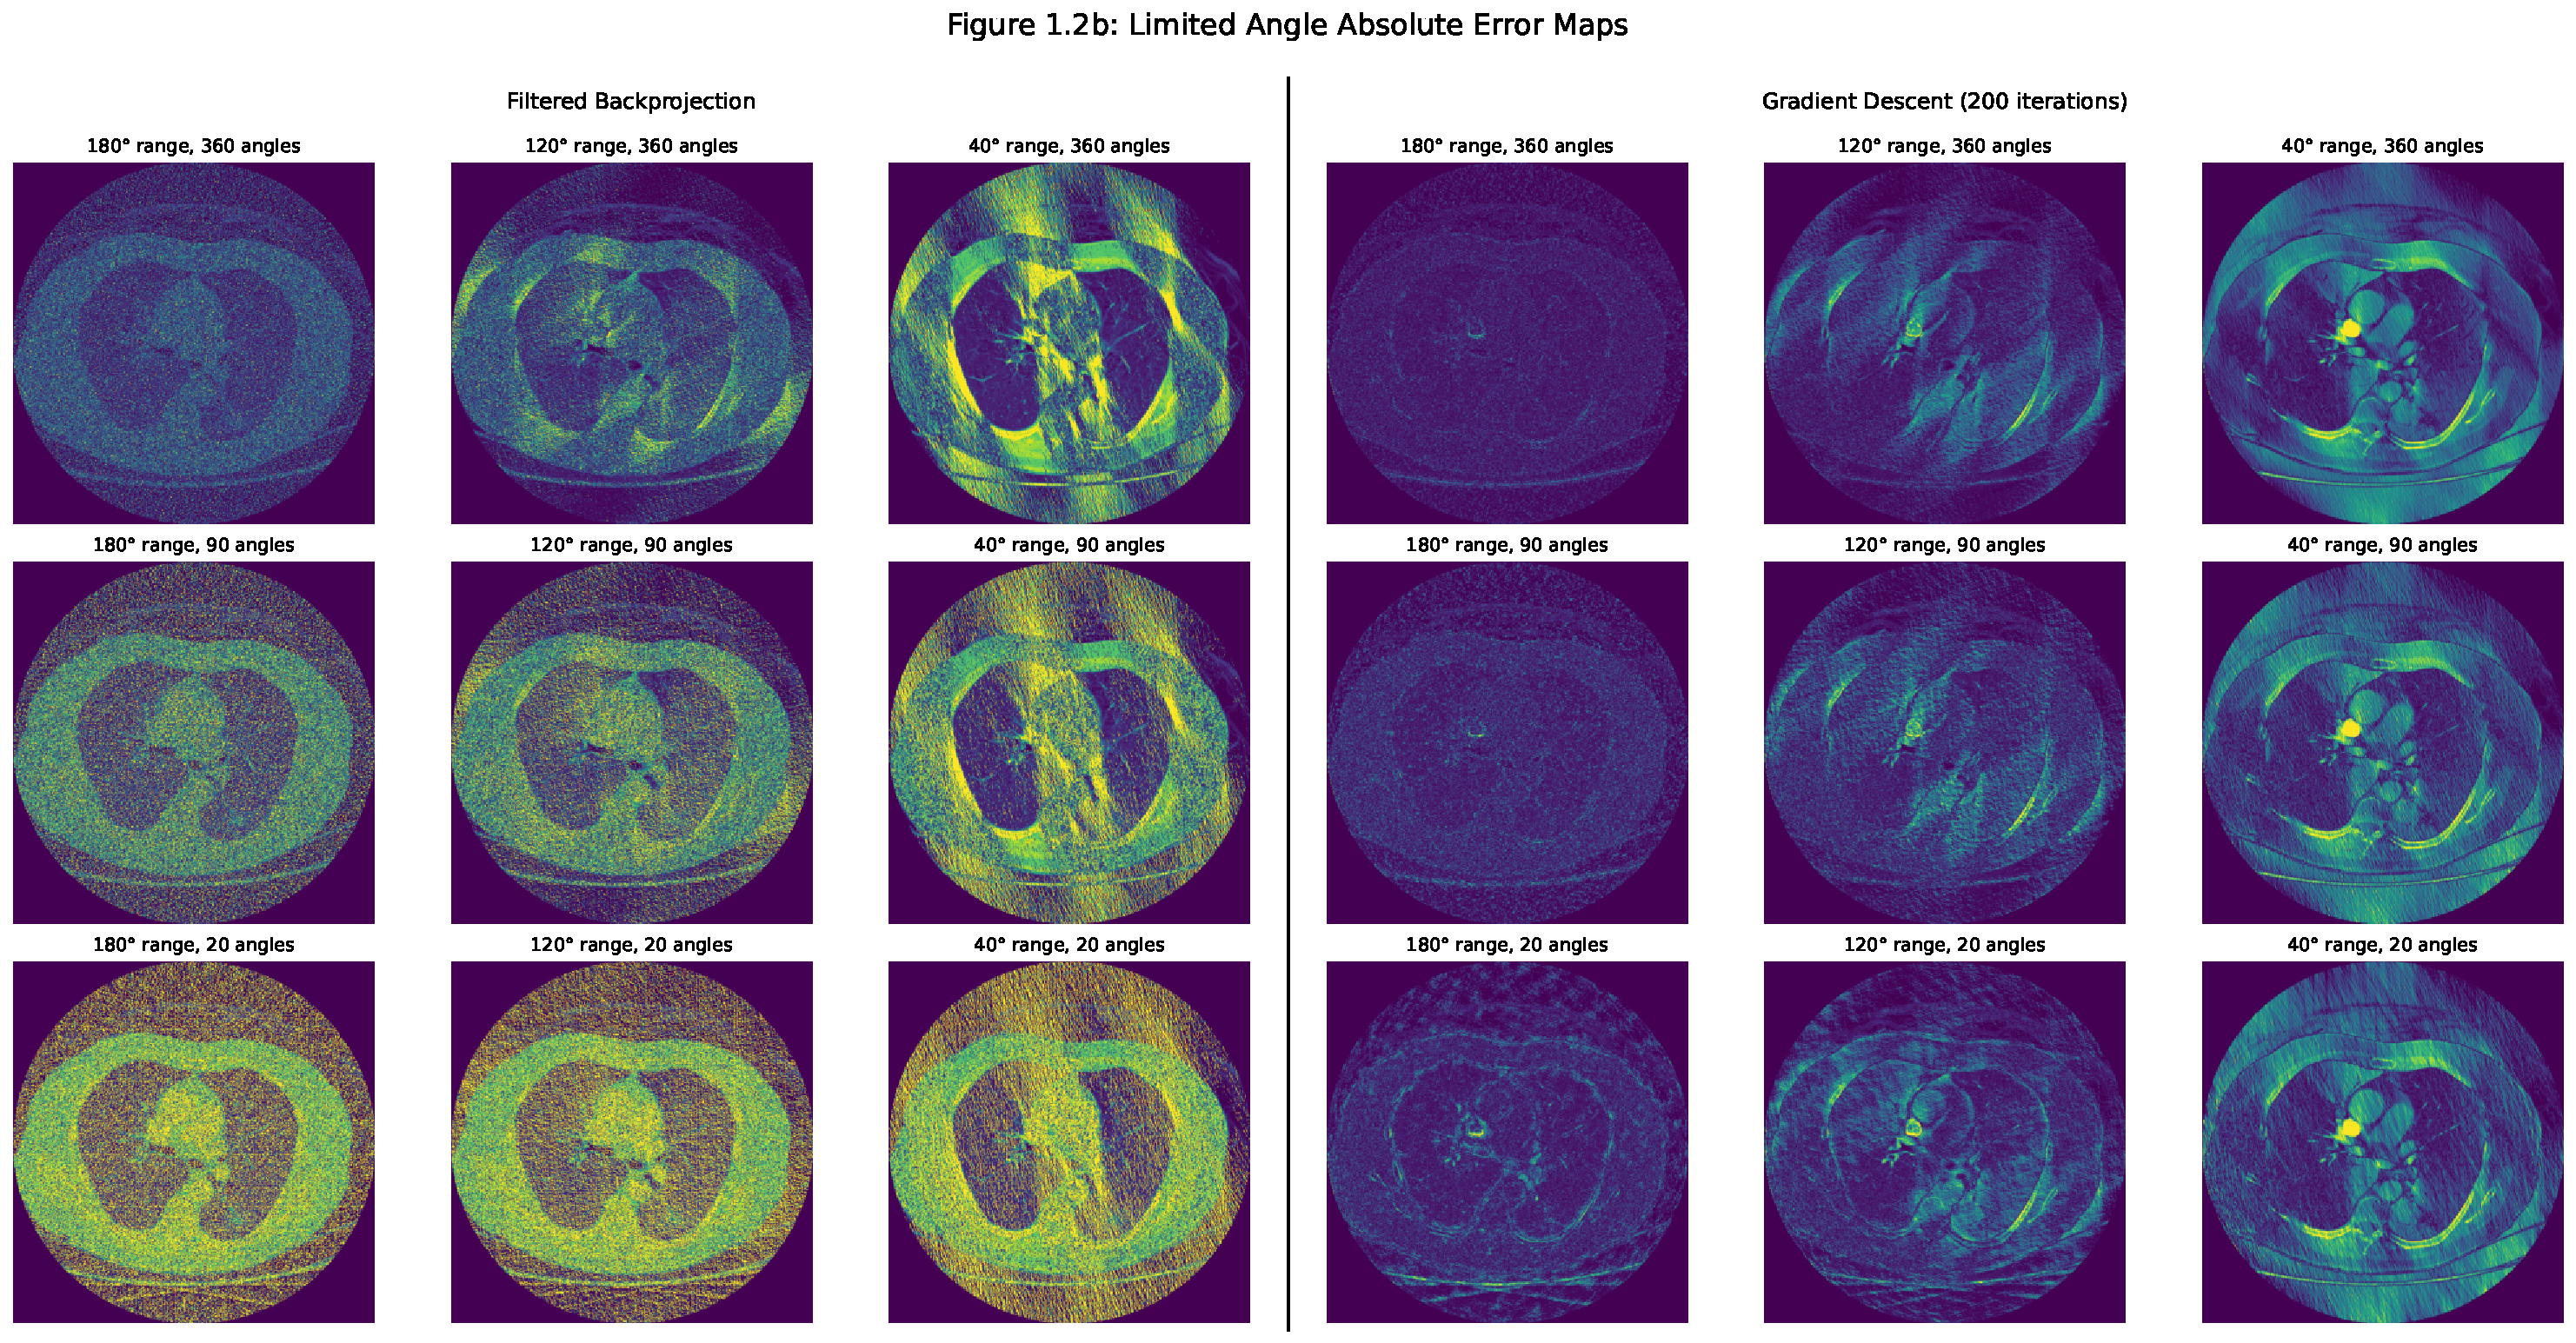
\includegraphics[width=0.9\textwidth]{figures/fig_1.2b_errors.pdf}
    \caption{Limited angle absolute error maps.}
\end{figure}

The Limited Angle case shows several key differences. In the FBP reconstructions, we see near perfect reconstructions at a range of 180, identical to Exercise 1.1. At a range of 120 degrees, FBP still recovers recognisable anatomy across all projections, however with some distortion of edges. This is a much better performance than for $I_0=10^3$ in Exercie 1.1, which was also the medium statistic. At the 40 degree range the reconstructions become unreadable due to streak artefacts running across the image in the direction corresponding to the measured anfular range. All three columns at this range are equally uninterpretable, similarly to the previous exercise, where all FBP reconstructions at low dose were entirely dominated by noise. Despite this, the consistency across reconstructions shows that when we have a limited range, the number of projections will not improve the image as we cannot recover information that simply is not present in the data. \\

\noindent In the Gradient Descent reconstructions, we see that it is better suited to a dealing with a reduction in the angular range, producing readable reconstructions for all projections in the 120 degree range. The success of GD is confirmed by the metrics we recover, where PSNR is 24-25 dB and SSIM of 0.45-0.57, confirming that the anatomy is well recovered. Comparing this to the middle case in our low dose reconstructions, the PSNR and SSIM ranged between 10-13 dB and 0.19-0.20 respectively, which shows a clear improvement in the ability of Gradient Descent to reconstruct limited angle sinograms compared to low dose ones. At the 40 degree range, GD produces blurred images with visible streaks. While these streaks are smoother than FBP's, all three images produced at this range are equally unrecognisable. \\ 

\noindent The main difference to Exercise 1.1 is the nature of the degradation of the images. In 1.1 we were reducing dose, producing spatially uniform, random noise throughout the image, so it degraded everywhere equally. In 1.2, the degradation is structured and directional, where even in the 40 degree range, we can clearly see some edges, while others are completely covered with streaks in one direction. This arises from a lack of information, as edges whose normal falls outside of the measured range are invisible, and cannot be recovered regardless of the algorithm used, as they simply do not exist in the data. \\

\subsubsection*{(c) Mathematical principles}

The mathematical principal describing this is the Fourier Slice Theorem, which stated that a 1D fourier transform of the detector function (a projection) at an angle $\theta$ is the same as a line or radial slice through the origin of the 2D fourier transform of the image at the same angle. The more projections that we take, the more radial slices we obtain, and at a range of 180 degrees, (due to symmetry of a circle) we have anough radial slices to cover the entire domain and consttruct the full fourier representation of the image. At a limited range however, only the radial lines corresponding to the 40 degree wedge are populated with radial lines, and the rest of the fourier space is entirely empty. No reconstructive algorithm can recover information that is not in the data, which results in deficiencies, and regardless of how many projections we take in this range, there will be almost no improvement due to the data needed simply not being there. \\

\noindent As discussed in Lecture 11 (02/03/2026), edges appear when there is a sharp change in the brightness or intensity in the image. We characterise them using the image gradient, where the gradient vector points in the direction of maximum intensity change, and its magnitude is largest at an edge. Therefore, the direction of an edge is perpendicular to the direction of the gradient vector. Connected with the Fourier Slice Theorem, an edge will only be visible in CT ifthe projection angle perpendicular to it lies withinthe measured range. This is precisely why edges disappear at limited angle ranges, as for a 40 degree range, only edges that are perpendicular tothe projections taken there will show up inthe reconstruction, and all others will be invisible regardless of how many projections we take or which reconstruction algorithm is used. \\

% ──────────────────────────────────────────────
\subsection*{Exercise 1.3: Reconstruction}

\subsubsection*{(a) FBP filters}

The available filters in \texttt{scikit-image} are: ramp (Ram-Lak), Shepp-Logan, cosine, Hamming, and Hann. 

\subsubsection*{(b) Filter comparison}

The Shepp-Logan and cosine filters were compared against Ram-Lak on the $I_0=10^3$, 360-angle sinogram.

\begin{figure}[H]
    \centering
    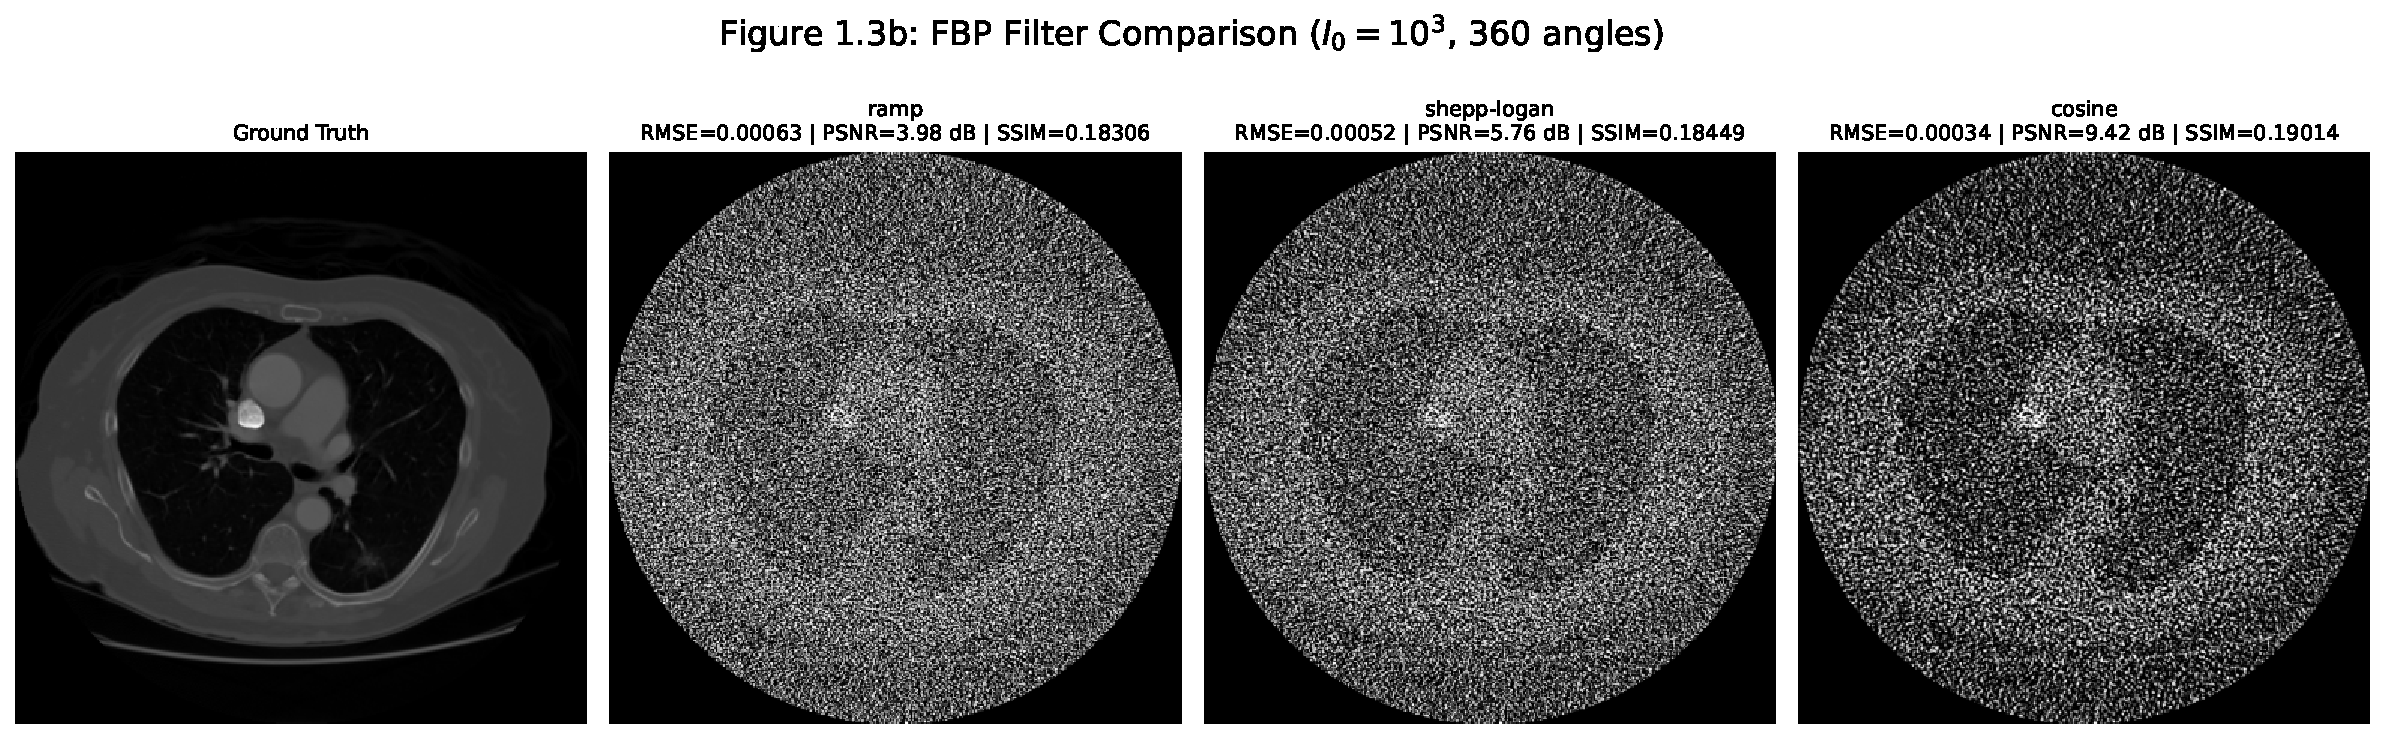
\includegraphics[width=0.95\textwidth]{figures/fig_1.3b.pdf}
    \caption{FBP filter comparison at $I_0=10^3$, 360 angles.}
\end{figure}

\noindent Moving from Ram-Lak to Shepp-Logan to cosine, RMSE decreased from 0.00063 to 0.00034 and PSNR increased from 3.98~dB to 9.43~dB, demonstrating increasing high-frequency attenuation. The cosine reconstruction is visibly less grainy, though SSIM values remain similar (0.18--0.19), indicating that while signal quality improves, structural similarity to ground truth is limited at this dose. Ultimately, no filter can fully compensate for insufficient photon counts in low-dose CT.

\subsubsection*{(c) OS-SART vs SIRT comparison}

OS-SART splits projections into $N$ subsets, performing $N$ updates per outer iteration. For fair comparison with 200-iteration SIRT, OS-SART used 10 subsets of 20 iterations (matching total forward/backward projection pairs).

\begin{figure}[H]
    \centering
    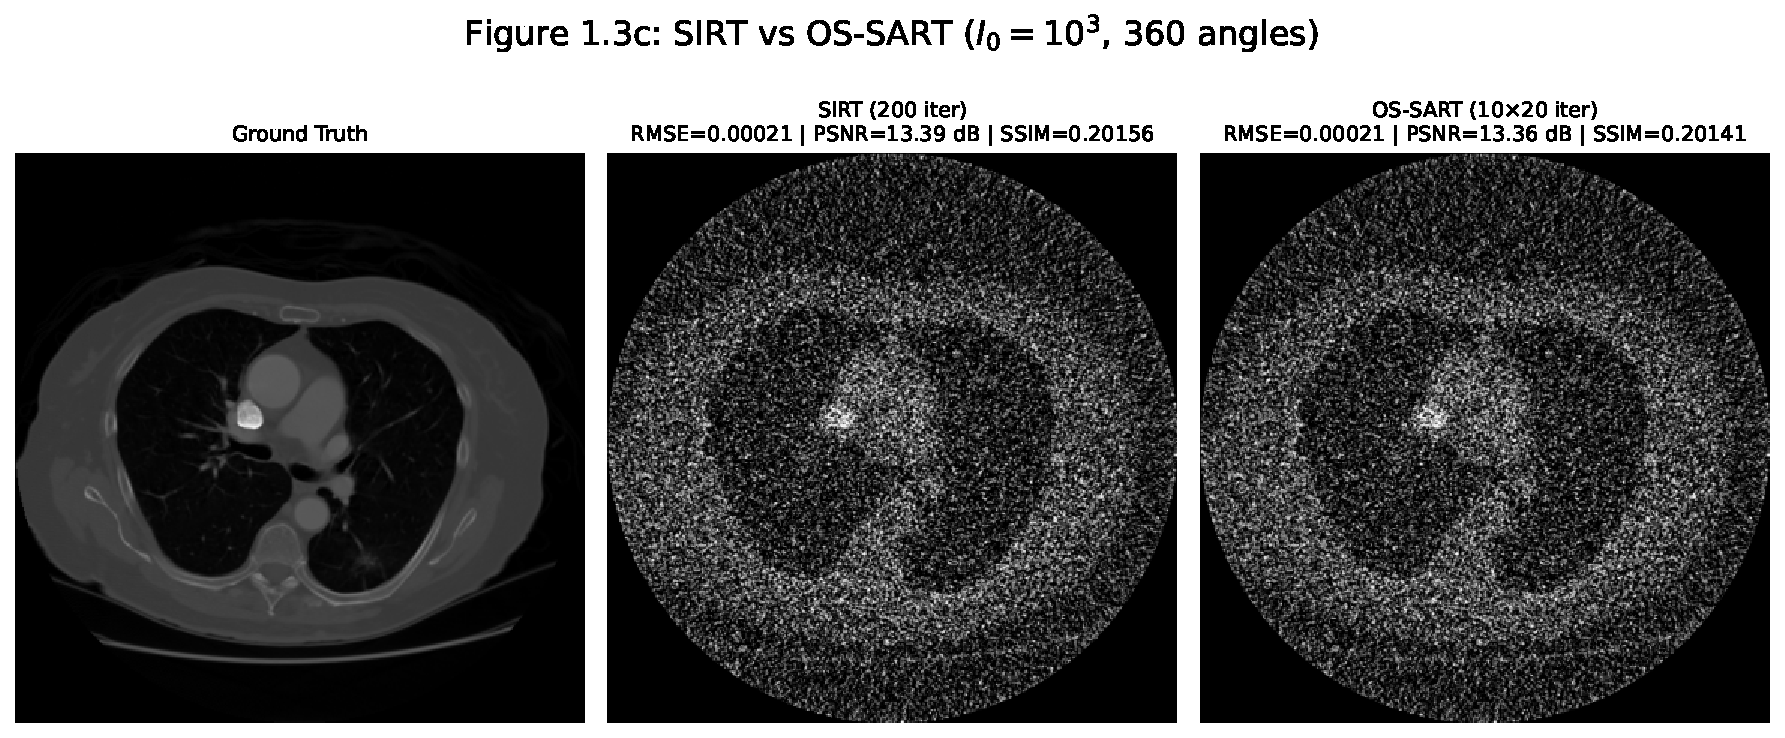
\includegraphics[width=0.95\textwidth]{figures/fig_1.3c_comparison.pdf}
    \caption{SIRT vs OS-SART reconstruction comparison.}
\end{figure}

\begin{figure}[H]
    \centering
    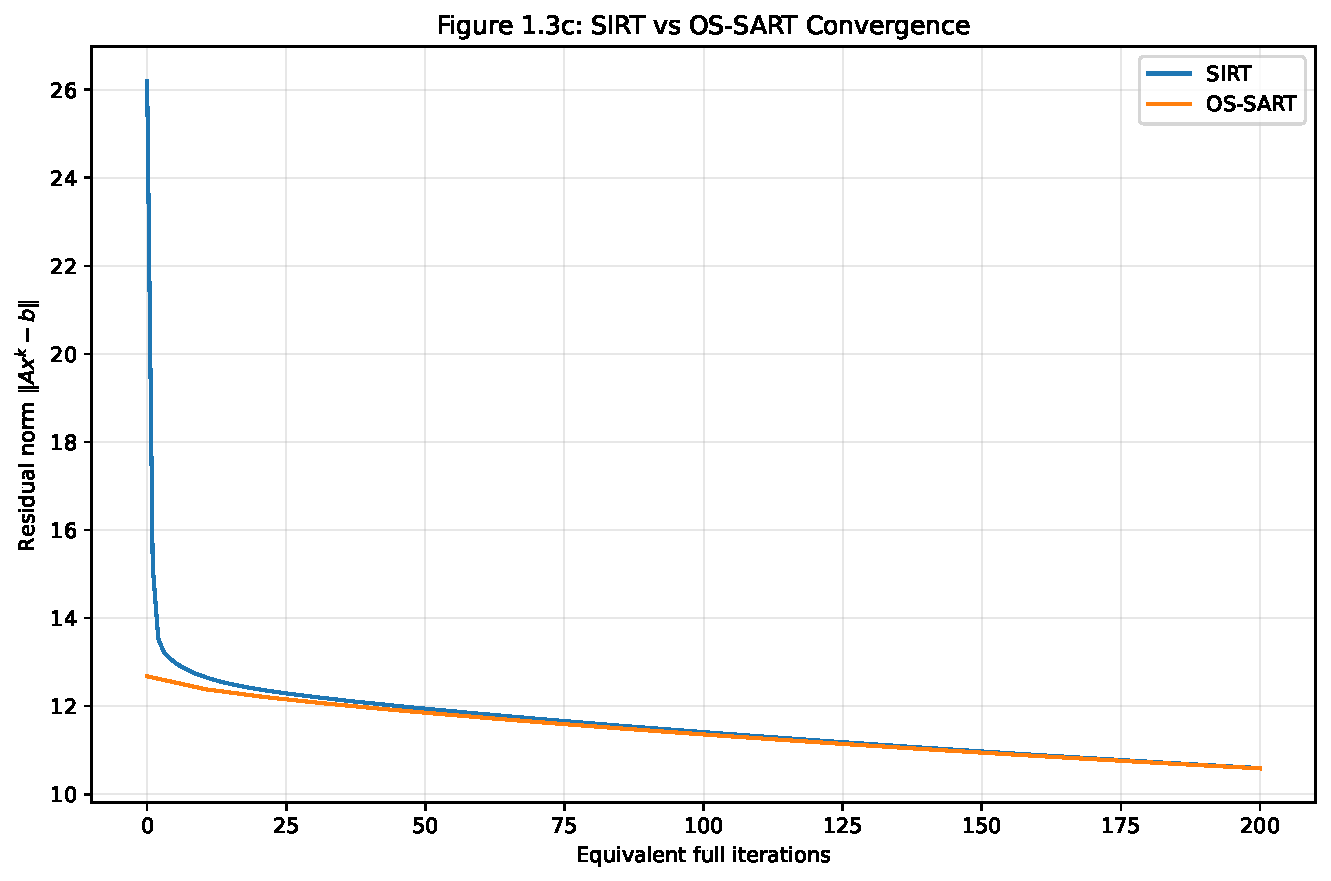
\includegraphics[width=0.7\textwidth]{figures/fig_1.3c_convergence.pdf}
    \caption{SIRT vs OS-SART convergence curves.}
\end{figure}

\noindent Both methods produce near-identical final reconstructions (RMSE 0.00021, PSNR $\approx$13.4~dB, SSIM $\approx$0.20), as expected since they solve the same minimisation problem. The convergence plot shows OS-SART's advantage: it reaches a low residual much faster because it completes the equivalent of 10 SIRT iterations in one pass through the data. SIRT takes approximately 20 iterations to reach the residual at which OS-SART begins. After this initial advantage, both curves converge to the same final residual. OS-SART's subset updates are individually noisier, but this averages out over time.

\subsubsection*{(d) MLEM/OSEM vs SIRT}

Both CT and PET reconstructions can be framed as minimisation problems, however the type of noise encountered in each type of imaging is different, meaning that the algoriths used for reconstructions will also differ. \\

The forward model in CT is $p = -\log(\frac{I}{I_0}) = \sum_i \mu_i l_i$, where the dominant noise is a mix of predominantly electronic Gaussian noise and Poisson photon counting noise (which also approximates to a Gaussian at high photon counts). The maximum likelihood estimate for Gaussian noise is obtained using least squares, which is the minimisation used in Gradient Descent (SIRT) algorithms.\\

PET detects individual photon pairs from positron annihilation events. This is a discrete counting process where the acquisition model is $I_j^{em} = \sum_i I_i l_{ij}$, and $I_j^{em}$ is the number of detected photon pairs along the line of response $j$. Because PET is counting individual events, its noise follows a Poisson distribution, and the data is very noise, with additional complexity from randomness, scatter events, detector calibration and pile up factors. Due to the nature of the noise, we cannot use a least squares minimisation, but maximise using the Poisson log likelihood. The MLEM (Maximum Likelihood Expectation Maximisation) and OSEM (Ordered Subsets Expectation Maximisation) algorithms do exactly that.\\

MLEM uses a multiplicative update rather than the additive step used in SIRT, which naturally controls non-negativity and correctly accounts for the Poisson statistics of the measurements, whereas OSEM is the ordered subset version of MLEM, the PET equivalent of using OS-SART in CT. It splits data into subsets to accelerate the convergence of the MLEM algorithm, providing a good reconstruction faster than MLEM.\\

In summary, we use MLEM and OSEM in PET because the reconstruction algorithm must match the noise model of the data. While CT is mainly Gaussian and therefore suits SIRT like algorithms, PET measurements are dominated by Poisson noise, requiring a statistically correct algorithm that reflects this.

% ──────────────────────────────────────────────
\section*{Module 2: MRI Image Denoising}
% ──────────────────────────────────────────────

\subsection*{Exercise 2.1: Visualisation and Identifying Noise}

\subsubsection*{(a) Loading data}

The complex k-space data was loaded from \texttt{knee.npy}. 

\subsubsection*{(b) K-space magnitude}

\begin{figure}[H]
    \centering
    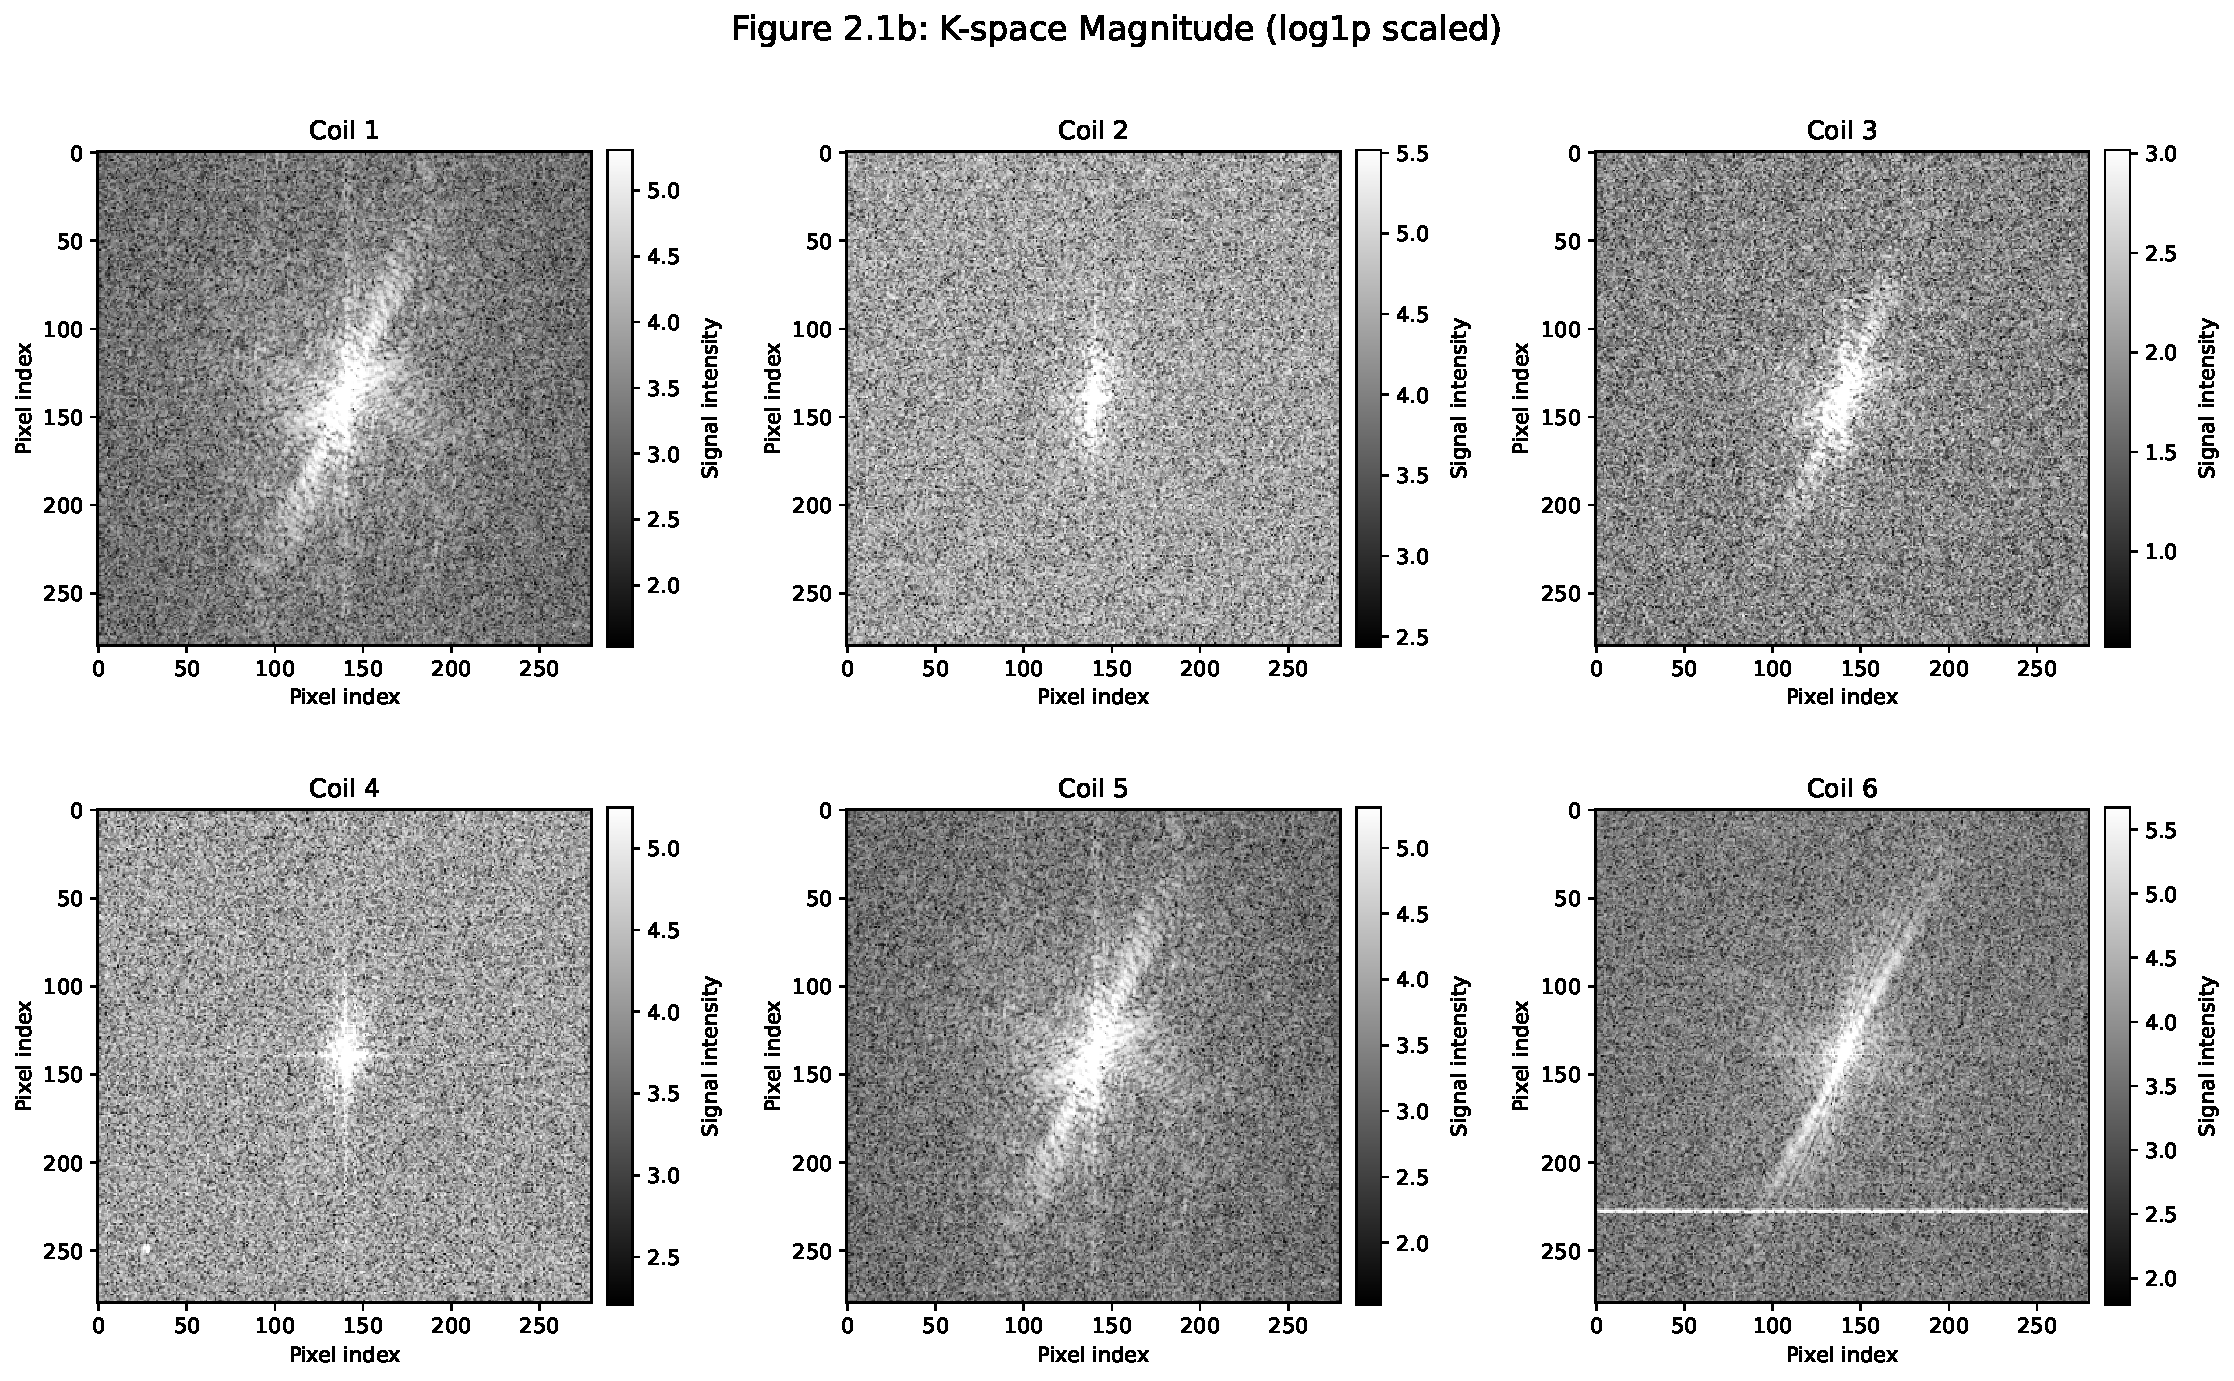
\includegraphics[width=0.95\textwidth]{figures/fig_2.1b.pdf}
    \caption{Log-scaled k-space magnitude for all six coils.}
\end{figure}

\subsubsection*{(c) Image space: magnitude and phase}

The data was transformed to image space using the 2D inverse FFT applied independently to each coil.

\begin{figure}[H]
    \centering
    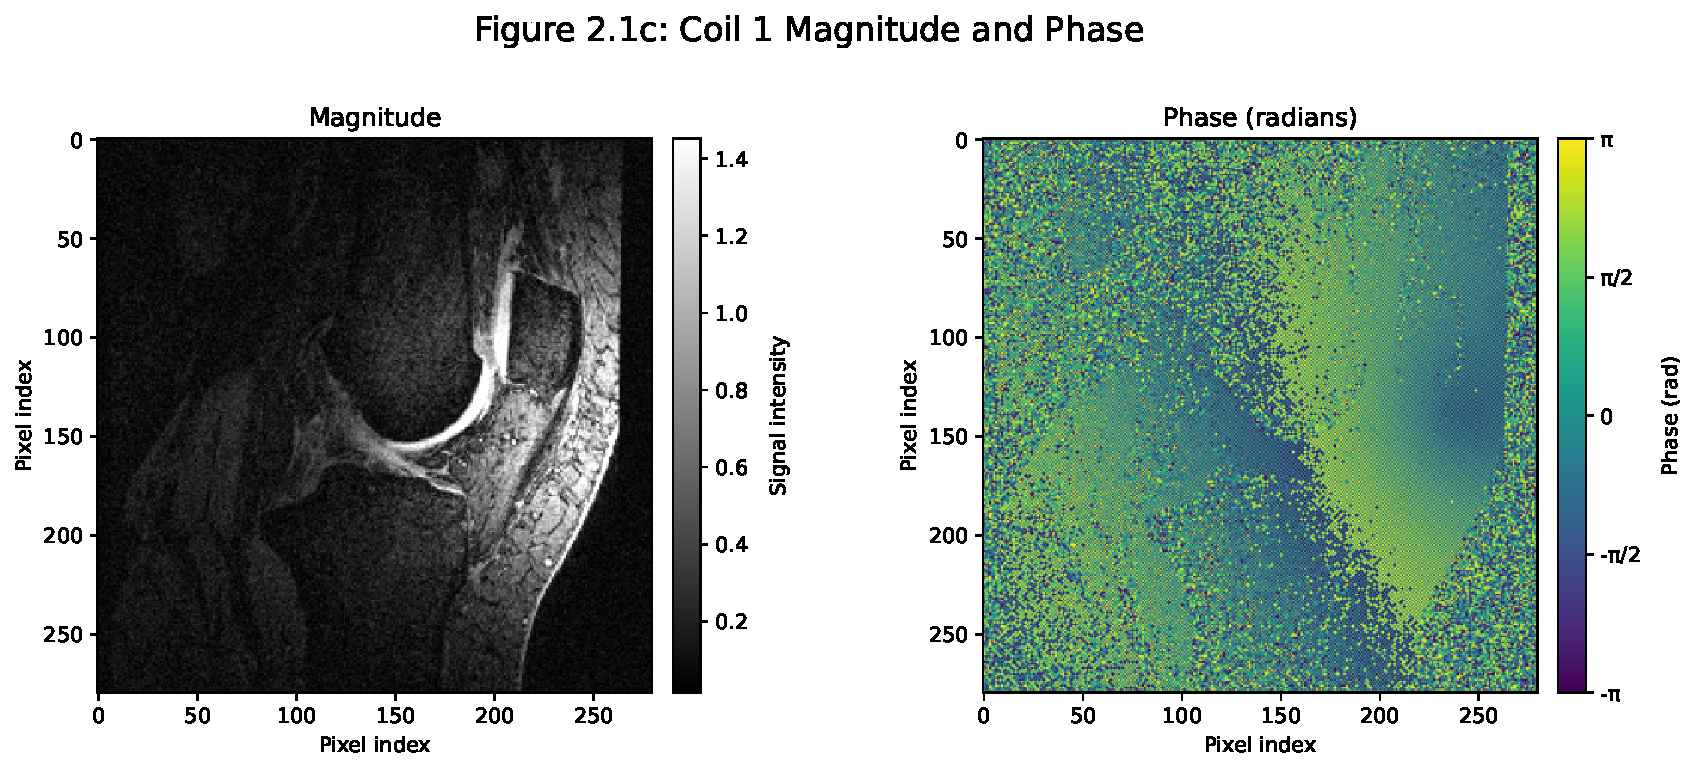
\includegraphics[width=0.85\textwidth]{figures/fig_2.1c.pdf}
    \caption{Magnitude and phase images from coil~1.}
\end{figure}

\noindent The magnitude plot shows signal intensity brightest where the coil is most sensitive to the underlying tissue. The phase shows smooth gradients across the tissue region, with random salt-and-pepper noise in the background where signal is near zero.

\subsubsection*{(d) All coil magnitude images}

\begin{figure}[H]
    \centering
    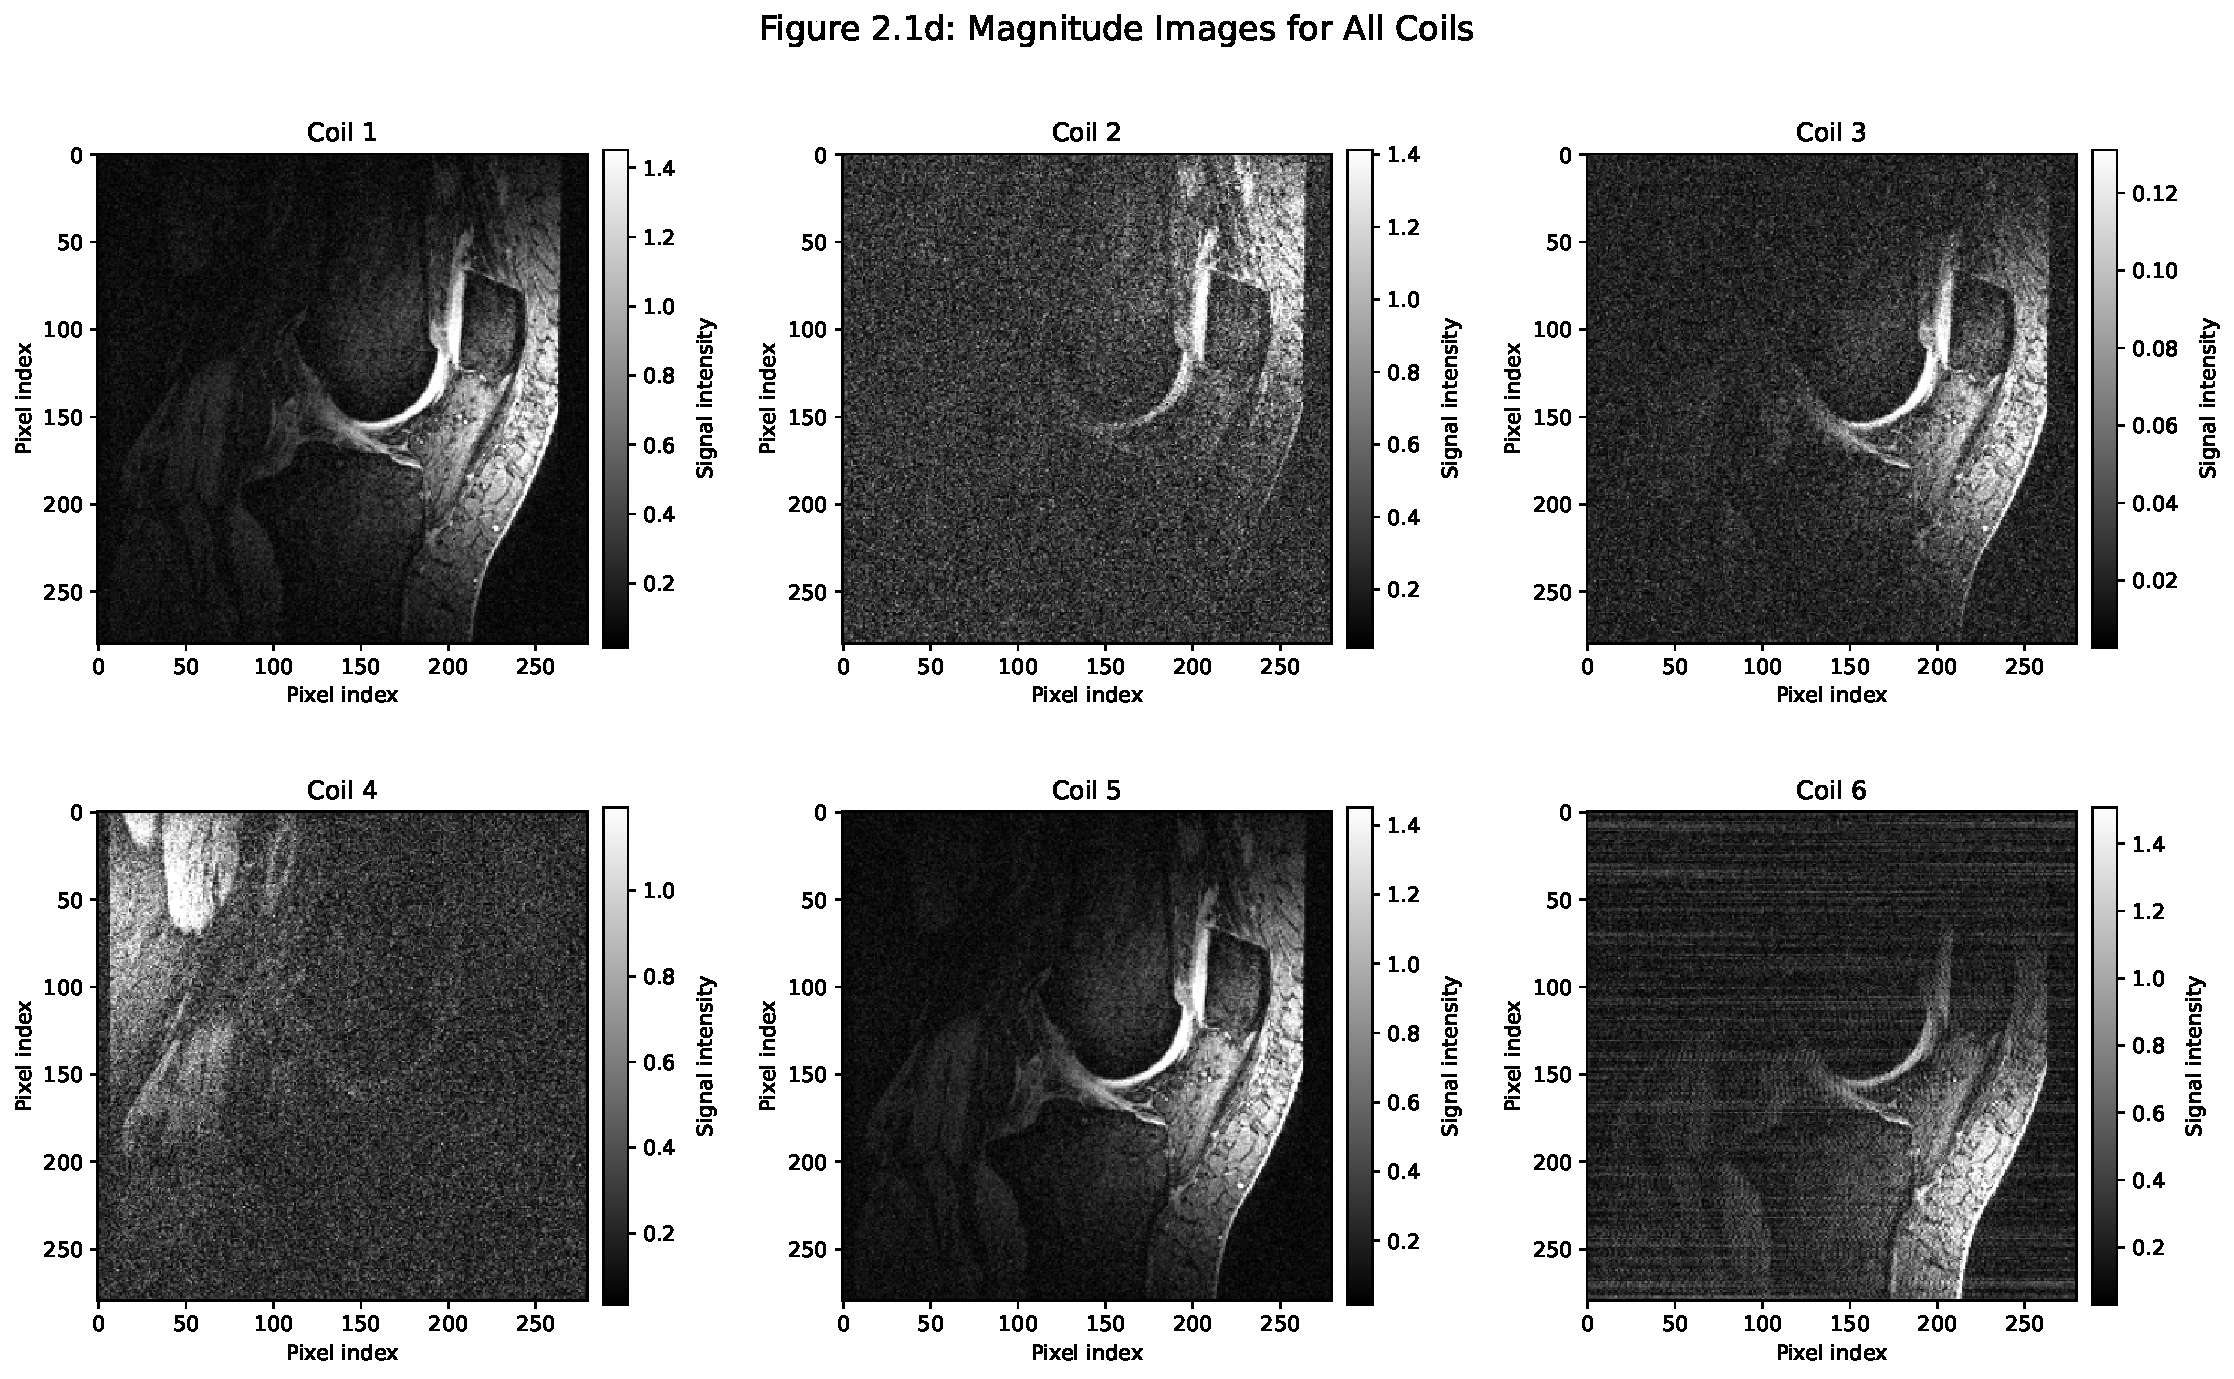
\includegraphics[width=0.95\textwidth]{figures/fig_2.1d.pdf}
    \caption{Magnitude images for all six coils.}
\end{figure}

\noindent Each coil shows a different perspective of the knee.

\subsubsection*{(e) Coil combination}

The coils were combined using root-sum-of-squares

\begin{figure}[H]
    \centering
    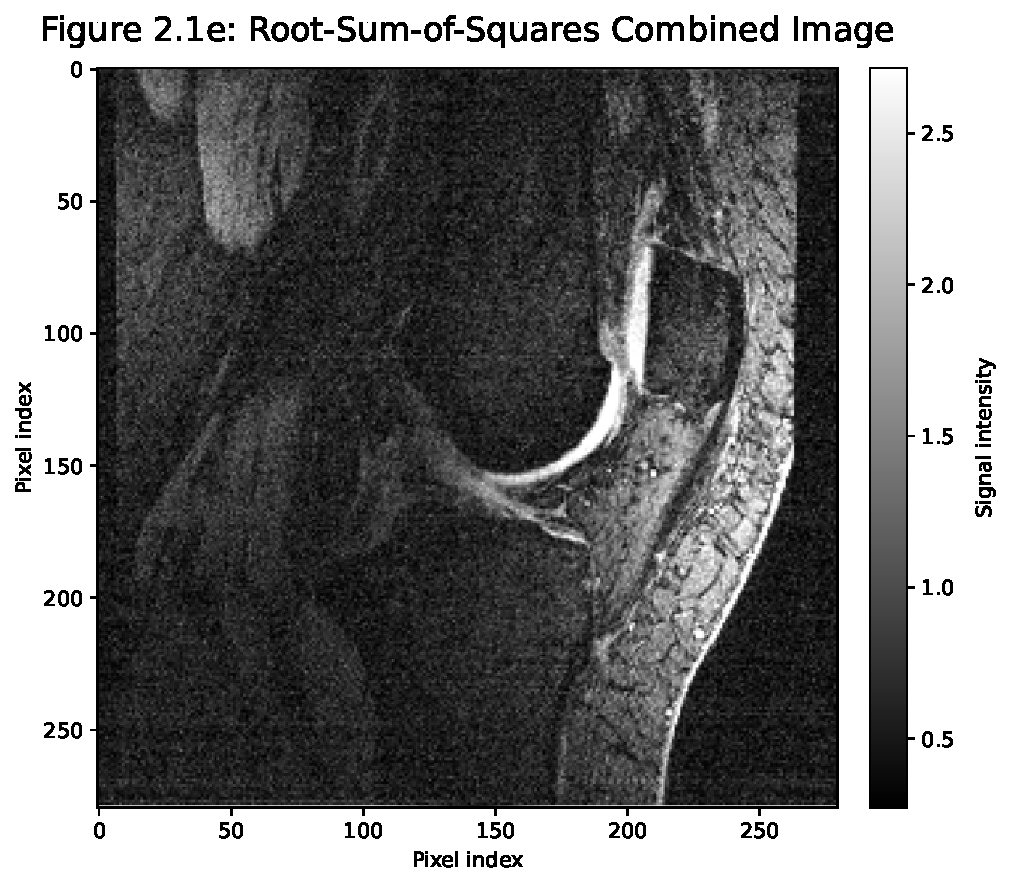
\includegraphics[width=0.6\textwidth]{figures/fig_2.1e.pdf}
    \caption{Root-sum-of-squares combined image.}
\end{figure}

\noindent The combined image shows more complete and uniform coverage compared to individual coils, with no cancellations from differing intensity ranges.

\subsubsection*{(f) Observations}

The k-space magnitude is visually similar across coils, with bright centres (low spatial frequencies encoding overall brightness) and rapidly decreasing signal towards edges (high frequencies encoding fine detail). \texttt{np.log1p()} scaling was necessary as the dynamic range is too large to visualise without it. Coil~6 shows a horizontal line artefact (likely a spike artefact from electrical discharge), and Coil~4 has a small artefact in the bottom left.

The image-space magnitudes show different regions of peak brightness corresponding to each coil's physical position, consistent with the sensitivity profiles described in lecture material. The combined rSoS image achieves uniform coverage without cancellations from differing intensity scales. The quality of Coils~4 and~6 is worse than the others, which may correspond to the artefacts observed in their k-space.

% ──────────────────────────────────────────────
\subsection*{Exercise 2.2: Removing Noise}

\subsubsection*{(a) Image denoising methods}

Gaussian ($\sigma=1$), bilateral ($d=10$, $\sigma_{\text{color}}=0.2$, $\sigma_{\text{space}}=8$), and wavelet (BayesShrink) filters were applied to the magnitude images from all coils.

\begin{figure}[H]
    \centering
    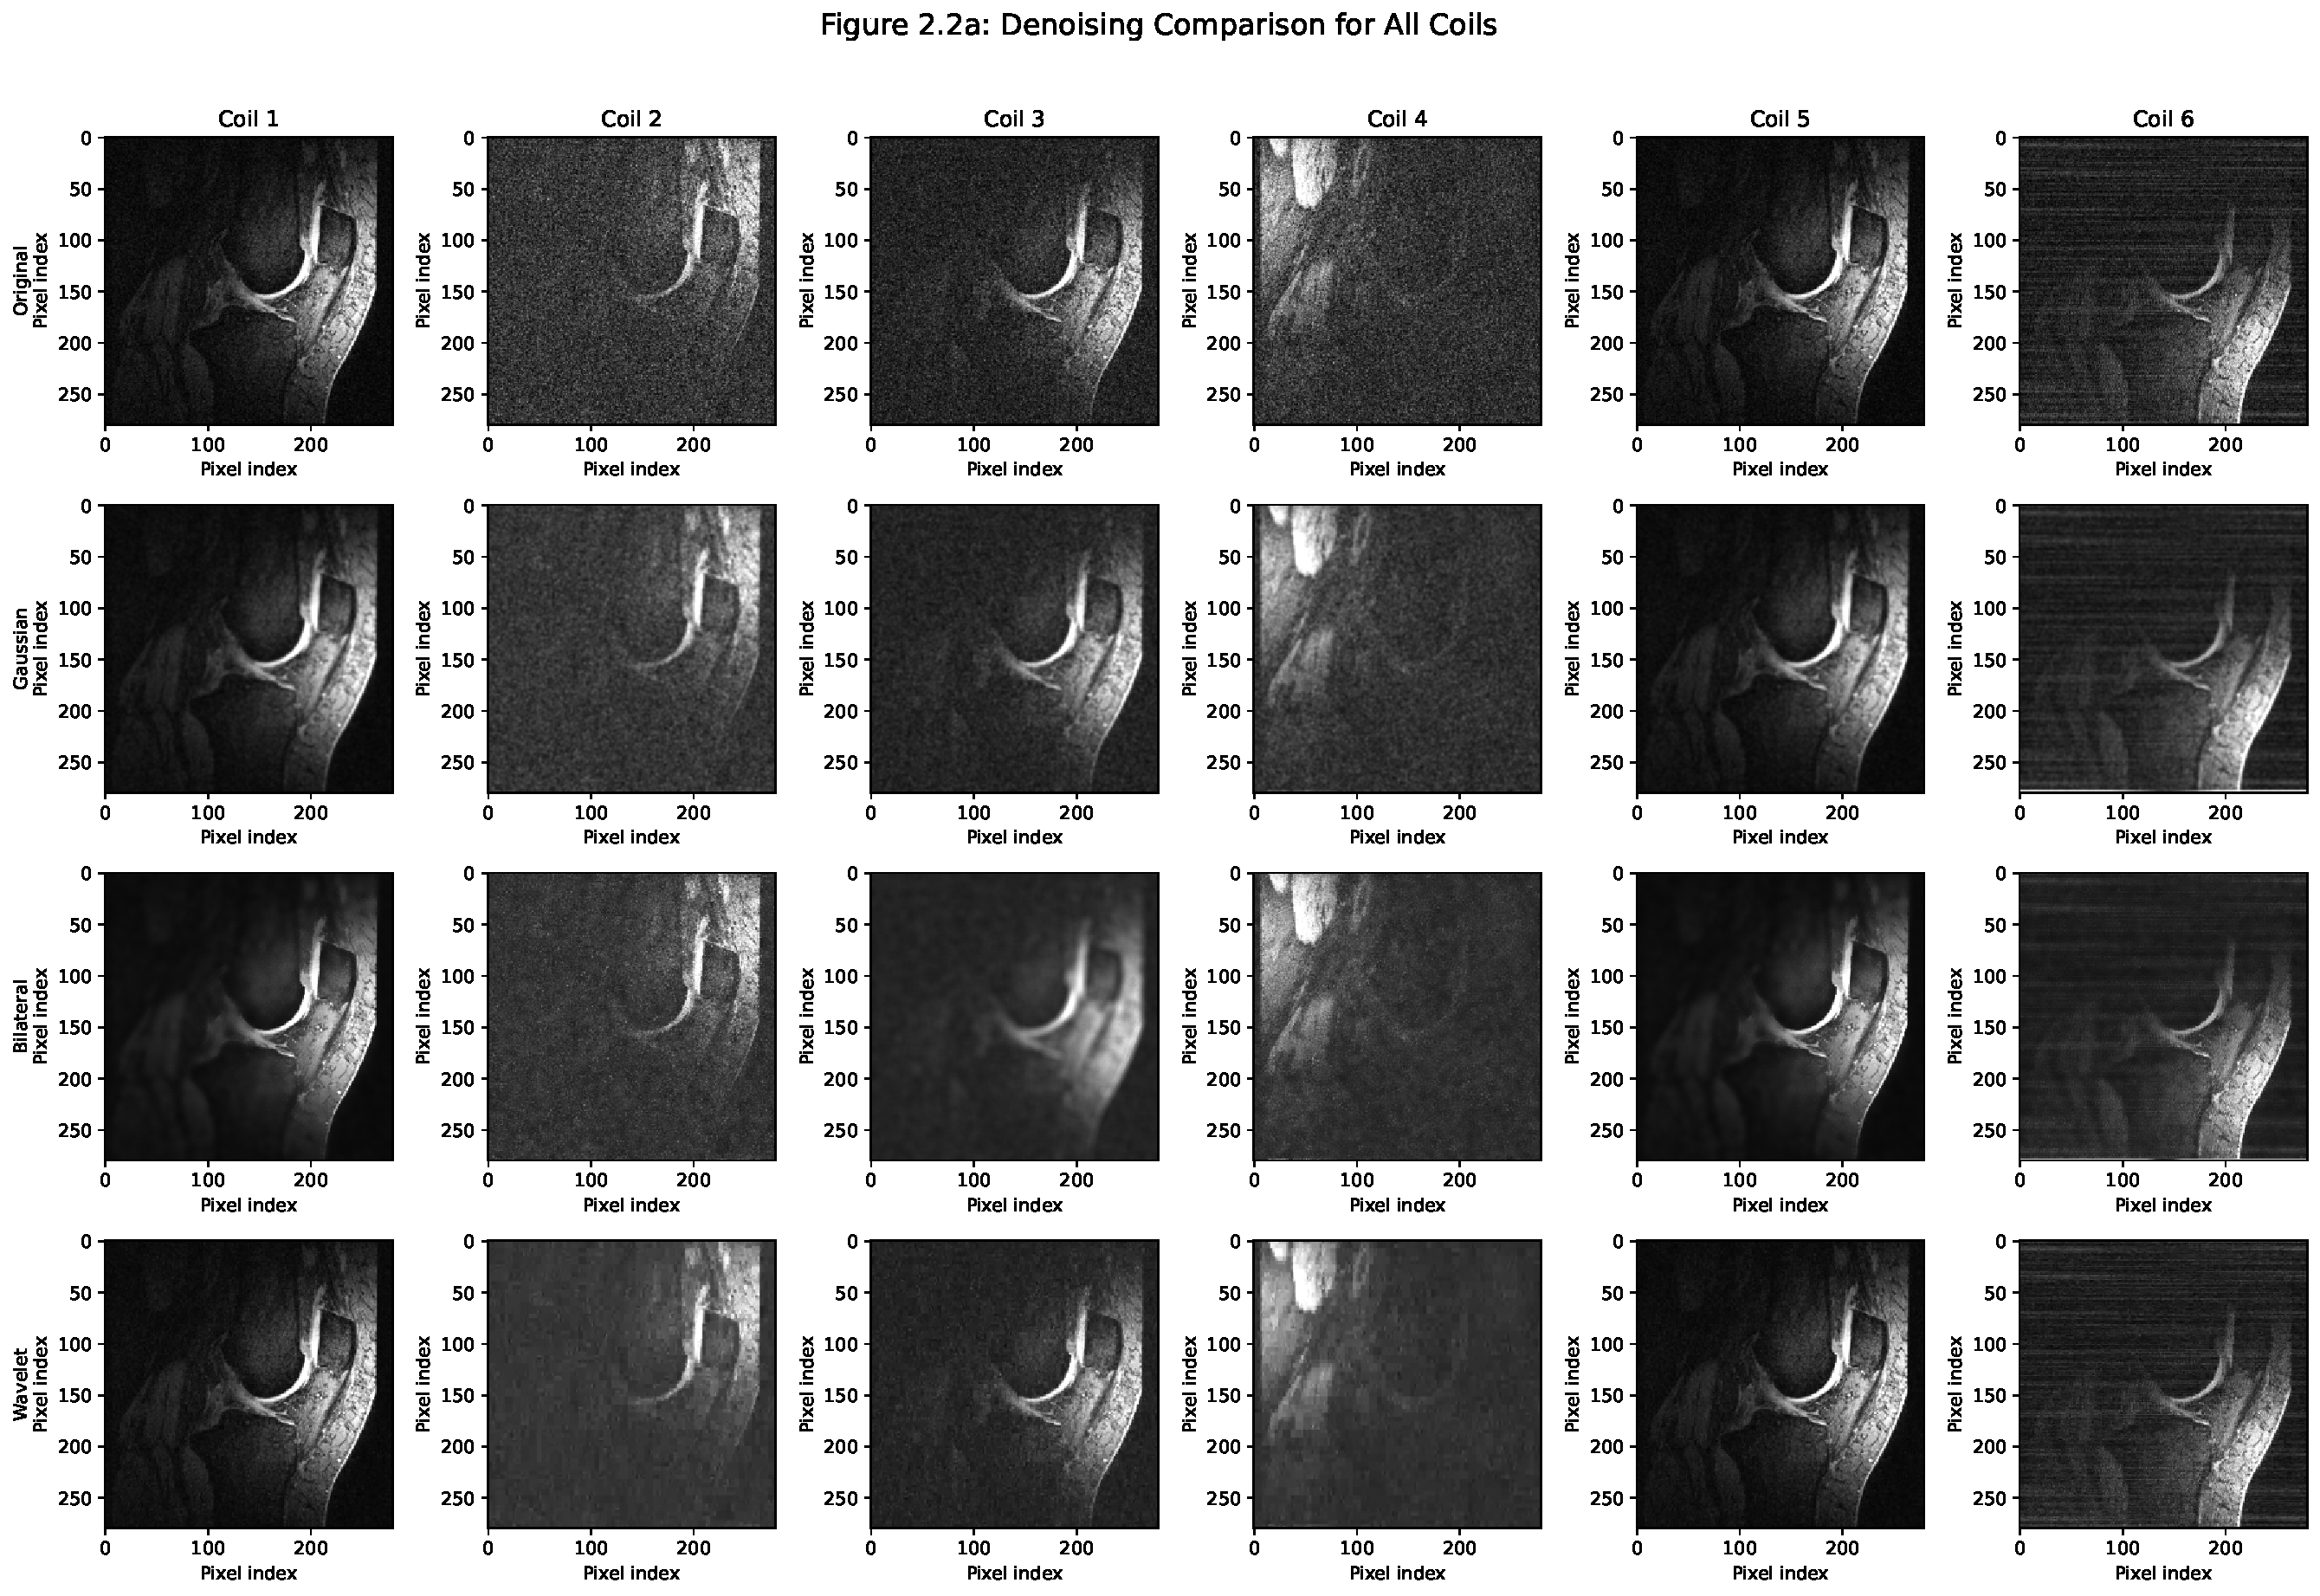
\includegraphics[width=0.95\textwidth]{figures/fig_2.2a.pdf}
    \caption{Denoising comparison across all coils: original, Gaussian, bilateral, wavelet.}
\end{figure}

\noindent Gaussian filtering reduced background noise consistently across coils but produced uniform smoothing that blurred edges, particularly visible in Coils~1 and~5. Bilateral filtering gave mixed results: it preserved edges well on Coils~1, 5, and~6, but struggled with Coil~3's low dynamic range ($\sim$0.02--0.12 versus $\sim$0.2--1.4 for other coils), highlighting its parameter sensitivity. Wavelet filtering was the most consistent, reducing background noise while preserving edge sharpness across all coils regardless of signal intensity range. None of the filters removed the diagonal streak artefact in Coil~6.

\subsubsection*{(b) Butterworth filter}

A Butterworth low-pass filter ($D_0=100$, $n=2$) was applied directly in k-space for the first coil. The filter attenuates frequencies beyond the cutoff: $H(u,v) = 1/(1 + (D/D_0)^{2n})$.

\begin{figure}[H]
    \centering
    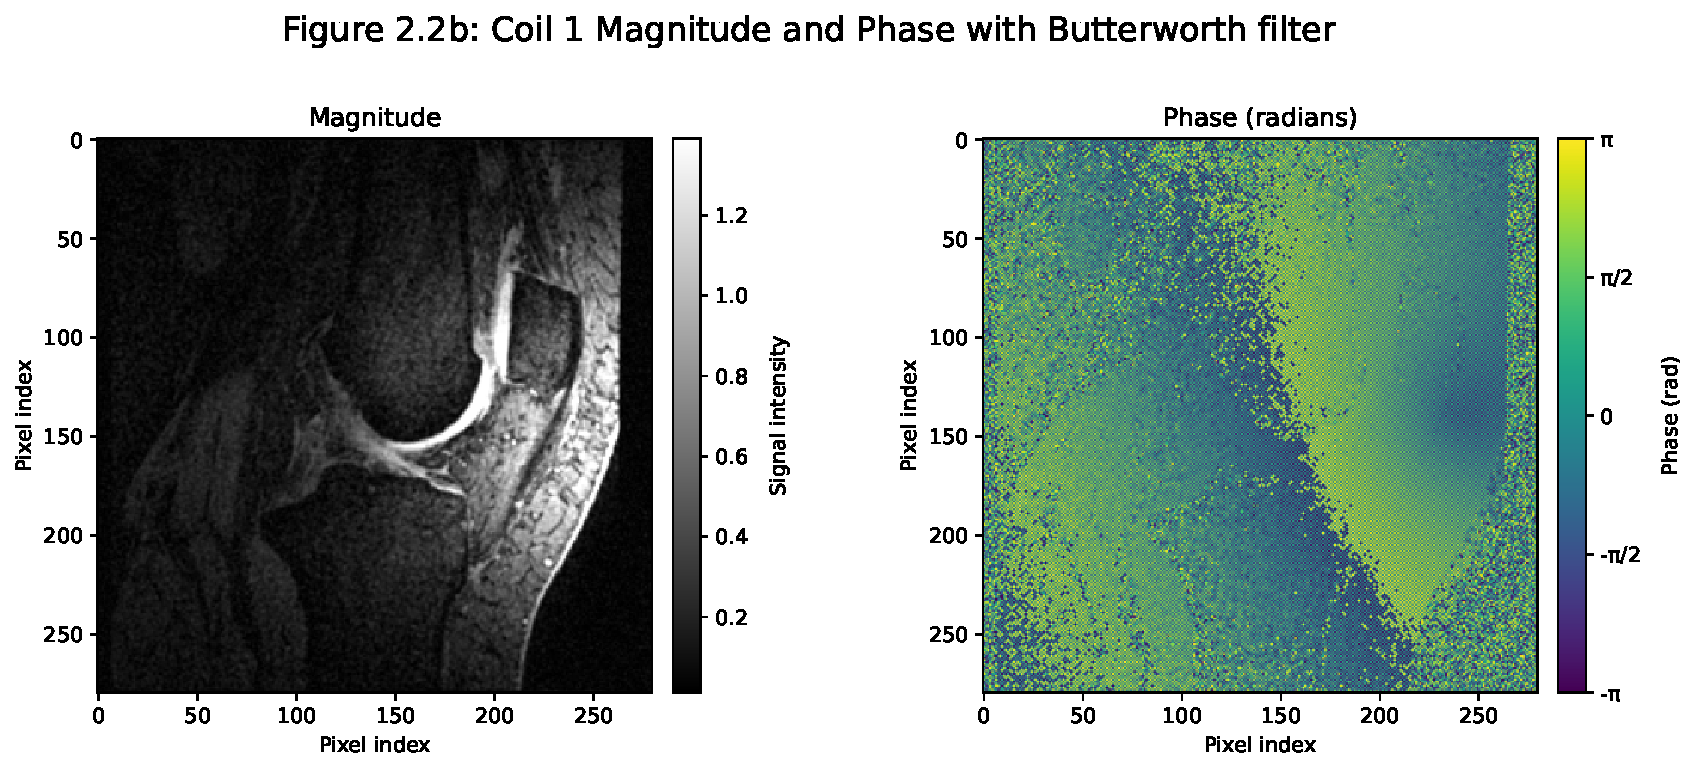
\includegraphics[width=0.85\textwidth]{figures/fig_2.2b.pdf}
    \caption{Butterworth-filtered magnitude and phase for coil~1 ($D_0=100$, $n=2$).}
\end{figure}

\noindent Unlike image-based methods, the Butterworth filter operates in k-space, attenuating high spatial frequencies before reconstruction. At $D_0=100$ (chosen after testing values of 10, 30, and 150), background noise was reduced while anatomical structures were preserved. The phase image shows smoother gradients than the unfiltered version. A disadvantage is that, like Gaussian filtering, it treats all high frequencies equally, and it can only be applied to one coil at a time.

\subsubsection*{(c) Denoised combined image}

Wavelet denoising was applied to the rSoS combined image, as it performed best across all coils.

\begin{figure}[H]
    \centering
    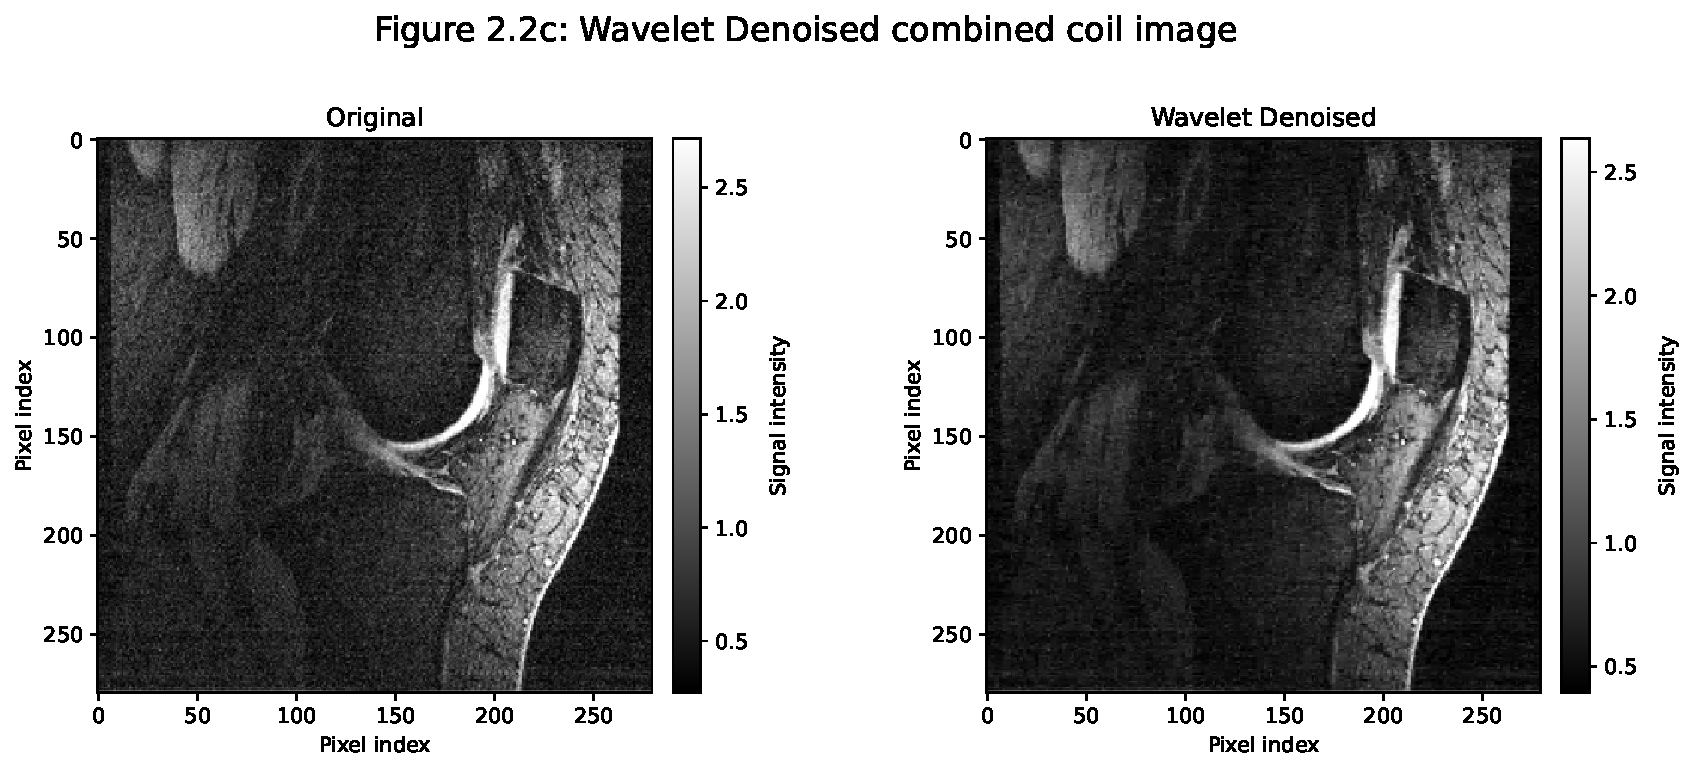
\includegraphics[width=0.85\textwidth]{figures/fig_2.2c.pdf}
    \caption{Original and wavelet-denoised combined image.}
\end{figure}

\noindent The denoised image shows reduced noise particularly in the dark regions, which appear more uniform with less speckle compared to the original.

\subsubsection*{(d) Discussion and further improvements}

Gaussian filtering is consistent but blurs edges uniformly, as it cannot distinguish noise from signal. Bilateral filtering extends this by weighting neighbours by intensity similarity, preserving edges in principle, but its performance is highly sensitive to parameters and it struggled with the low dynamic range of Coil~3. Wavelet filtering was the most robust, decomposing images into wavelet coefficients and applying adaptive soft thresholding per subband, effectively distinguishing noise from structural detail across all coils. The Butterworth filter operates in k-space and can target frequency-specific artefacts, but treats all high frequencies equally and is applied per-coil.

To further improve the combined image: (1)~applying the Butterworth filter to all six coils before rSoS combination would reduce noise at the source level; (2)~sensitivity-weighted coil combination (rather than equal-weight rSoS) would down-weight noisy coils in specific regions; (3)~deep learning methods could learn noise distributions from training data and produce cleaner reconstructions than classical methods.

% ──────────────────────────────────────────────
\section*{Module 3: Image Segmentation Methods}
% ──────────────────────────────────────────────

\subsection*{Exercise 3.1: Critical Comparison of Methods}

\subsubsection*{(a) Selected publications}

\begin{enumerate}
    \item \textbf{Non-ML/DL:} Khorshidi, A. (2023). Tumor segmentation via enhanced area growth algorithm for lung CT images. \textit{BMC Medical Imaging}, 23:189.
    \item \textbf{DL:} Kashyap, M. et al.\ (2025). Automated deep learning--based detection and segmentation of lung tumors at CT imaging. \textit{Radiology}, 314(1):e233029.
\end{enumerate}

\subsubsection*{(b) Summaries and critical comparison}

\textbf{Paper summaries:}

The Khorshidi (2023) paper presents an Enhanced Area Growth (EAG) algorithm to segment lung CT images. The method is a classical region-growing approach, where a point inside the tumour is chosen by the user and the algorithm expands outwards by checking the colour intensity values of neighbouring pixels, accepting points if they are similar within a threshold. The paper explores enhancements including contrast augmentation, local thresholding, multi-seed-point growth, and edge refinement. Tested on 60~CT scans across four databases, the EAG achieved a Dice coefficient of $0.92 \pm 0.03$ compared to $0.80 \pm 0.02$ for the basic algorithm, and an accuracy of 92.1\%.

The Kashyap et al.\ (2025) paper develops a 3D U-Net ensemble model for detecting and segmenting lung tumours on CT scans, trained on 1504 pre-radiotherapy CT simulation scans from 1295 patients. The ensemble combines two 3D U-Nets (one high-resolution with small input volume, one low-resolution with large input volume), achieving 92\% sensitivity and 82\% specificity in detection, and a median Dice of 0.77 for segmentation, near the interphysician Dice of 0.80. Segmentation took 76.6~seconds on average versus over 160~seconds for physicians. An exploratory evaluation on scans with multiple tumours achieved 67\% sensitivity.\\

\textbf{Critical comparison:}

Both papers tackle lung tumour segmentation on CT images. The EAG algorithm is semi-automatic, requiring a user to select the start point and maximum tumour radius. This requires anatomical knowledge and the quality of results remains partially dependent on the initial point selected. The deep learning model is entirely automatic, taking raw CT inputs and outputting detection and segmentation without guidance, a major advantage for workflows where manual interaction per scan is not feasible.

The EAG algorithm reports a higher Dice coefficient (0.92 vs 0.77), but these are not directly comparable. The EAG was evaluated on only 60 images with a single expert reference, whereas the deep learning model was evaluated on 100 images against three physician segmentations per scan. The EAG also uses a seed point that already locates the tumour, while the deep learning model must detect it first. The interphysician Dice of 0.80 provides a clear benchmark showing the model approaches expert-level performance.

Both methods face different challenges. The EAG algorithm cannot segment fragmented or multiple tumours due to its seed-point initialisation, and struggles when tumours encroach on the lung wall or are surrounded by tissue of similar density. The lung masking step mitigates but does not fully resolve this. The deep learning model struggled with very large tumours that could not fit within its 3D input patches, leading to underestimated volumes. However, the EAG algorithm performed better on large tumours as it is not patch-constrained and can freely interpolate between growth points. The deep learning model was trained on scans where not all tumours were consistently segmented, yet still demonstrated reasonable performance when evaluated on multi-tumour scans.

In terms of accessibility, the EAG algorithm works on a single image with minimal compute requirements. The deep learning model requires a large labelled dataset and GPU infrastructure for training, but once deployed segments tumours in roughly 77~seconds compared to an average of 170~seconds for physicians.

In summary, the EAG algorithm is simpler and achieves high accuracy on well-defined tumours when correctly initialised, but is semi-automatic, parameter-sensitive, and validated less rigorously with a single expert reference. The deep learning approach is evaluated more thoroughly with detection metrics, segmentation metrics, volume agreement analysis, timing comparisons, a negative control set, and benchmarking against three independent physicians. It requires more data and compute to develop, but once trained is fully automatic and approaches expert-level performance.

\subsubsection*{(c) Proposed improvements}

Focusing on the deep learning paper, there are several key areas for improvement. The 3D patch-based approach results in difficulties detecting and segmenting large tumours as they may not fit within a single patch. Implementing a coarse-to-fine pipeline could address this: a first-pass model operating on the entire CT volume or very large patches would roughly identify tumours, before a second-pass model refines the segmentation within cropped regions around each detection. This way, even very large tumours would be fully captured in the first pass.

Another improvement is addressing the training data labelling inconsistency. The training set contained scans where not all tumours were segmented (some were excluded from the radiation therapy plan), which means the model was sometimes shown scans where real tumours appeared as background, potentially teaching it to ignore them. This could be resolved by either exhaustively annotating all tumours, or masking out unlabelled tumour regions during training so the loss function does not penalise the model for detecting them. This would also improve the model's multi-tumour detection sensitivity, which currently sits at 67\%.

Incorporating PET data as an additional input channel would also be valuable, as the worst-performing cases all involved tumours invading the mediastinum or chest wall, where CT alone makes boundaries too ambiguous. PET highlights metabolically active tumour tissue and could disambiguate tumour from collapsed lung or adjacent structures, making the model better suited to challenging clinical cases.

% ──────────────────────────────────────────────
\section*{Declaration of Use of Autogeneration Tools}
% ──────────────────────────────────────────────

Autogeneration tools were used during this coursework to assist with understanding mathematical derivations, plot styling, checking and debugging code, cleaning up repository setup files, and formatting of markdown cells and \LaTeX. All code, explanations, and answers were written by myself and were not generated by these tools. Autogeneration tools were \textbf{not} used for Module~3.

\end{document}